\documentclass[a4paper,10pt]{report}

\usepackage[utf8]{inputenc}
\usepackage{xspace}
\usepackage{graphicx,graphics} 
\usepackage{color}
\usepackage{amsmath}
\usepackage{amsfonts}
\usepackage{amssymb}
\usepackage{amsthm}
\usepackage{algorithm}
\usepackage{algorithmic}
\usepackage{longtable}
\usepackage{complexity}
\usepackage{tkz-graph}
\usepackage{float}
\usepackage{setspace}
\renewcommand{\algorithmicrequire}{\textbf{Input:}}
\renewcommand{\algorithmicensure}{\textbf{Output:}}
  
\graphicspath{{figures/}}
\newcommand\rmatching{${\cal R}$-matching\xspace}
\newcommand\mdelay{$\cal M$-delay\xspace}
\newcommand\matchedgraph{{\bf matched graph}}

\newcommand{\reporttitle}{Latency management for Deterministic Networking}     % Titre
\newcommand{\reportauthor}{Maël \textsc{Guiraud }} % Auteur
\newcommand{\reportsubject}{Graduation Memory} 
\newcommand{\HRule}{\rule{\linewidth}{0.5mm}}
\setlength{\parskip}{1ex} % Espace entre les paragraphes

\newcommand{\todo}[1]{}
\renewcommand{\todo}[1]{{\color{red} TODO: {#1}}}
\begin{document}
\begin{titlepage}

\begin{center}



\begin{minipage}[t]{0.48\textwidth}
  \begin{flushleft} \large
       
\includegraphics [width=50mm]{logo.png} \\[0.5cm]
  \end{flushleft}
\end{minipage}
\begin{minipage}[t]{0.48\textwidth}
  \begin{flushright} \large
    
\includegraphics [width=50mm]{logon.png} \\[0.5cm]
  \end{flushright}
\end{minipage}
 \\[3cm]

\textsc{\Large \reportsubject}\\[0.5cm]
\HRule \\[0.4cm]
{\huge \bfseries \reporttitle}\\[0.4cm]
\HRule \\[1.5cm]

\begin{minipage}[t]{1.0\textwidth}
  \begin{center} \large
    \emph{Master 2  :} 
   Algorithmique et Modélisation à l'Interface des Sciences( AMIS) \\

  \end{center}
  \end{minipage}
  \\[3cm]
 
\begin{minipage}[t]{0.3\textwidth}
  \begin{flushleft} \large
    \emph{Student :}\\
    \reportauthor 
  \end{flushleft}
\end{minipage}
\begin{minipage}[t]{0.6\textwidth}
  \begin{flushright} \large
    \emph{Supervisors :} \\
    Mr.Dominique \textsc{Barth} \\
    Mr.Olivier \textsc{Marcé} \\
    Mr.Yann \textsc{Strozecki} \\
    Mr.Christian \textsc{Cadéré} \\

  \end{flushright}
\end{minipage}

\vfill

{\large September 2016}

\end{center}

\end{titlepage}

\newpage
\null
\newpage
\tableofcontents

\begin{chapter}{Context, company and subject}
\begin{section}{Company}
 Description de Nokia Bell Labs, Activité dans les équipements télécoms. (Voir avec Olivier)
\end{section}
\begin{section}{Context}
Current mobile network architecture consist in distributed radio access networks.
The evolutions proposed in next generations aim centralised radio network architectures (C-RAN) to reduce consumption costs 
and power at the base stations. These C-RAN architectures include simplified base stations at each antenna (Remote Radio Heads: RRH) 
and central processing units (baseband unit: BBU) located in the cloud. Thus, this type of architecture confronts the problem of mastering 
the latency in the transfer process.  Low latency is considered critical for the 5G, in particular for the deployment of C-RAN approach 
(allowing time constraints like HARQ to be fulfilled over non dedicated networks), or to reach E2E expected latency from 1 to 10ms 
(depending on targeted services). One specificity in the C-RAN context is not only the latency constraint, but also the periodicity of 
the data transfer between RRH and BBU.  New scheduling and routing paradigms and new technologies have to be considered to  gurantee 
delay constrained periodic data transfers. Dynamical optical bypass and dynamical management of the emission should be considered to
guarantee latency constraints. This is why this study is a contribution to the ANR project N-Green.

N-GREEN proposes a new type of switching/routing node and a specific network architecture exploiting WDM packets thanks to a new generation of optical add/drop multiplexers (WSADM: WDM slotted add/drop multiplexer). These packets having a fixed duration close to 1 µs are transported in a transparent way, to better exploit the switching matrix of the node; their headers will be transported over one dedicated wavelength at a lower bit rate, to reduce the physical constraints of the electronic processing and scheduler.

 Thus, this subject targets new scheduling and routing paradigms to solve this periodic and delay constrained data transfert.
 Indeed, one of the most promising approaches relies to the concept of Deterministic Networking (DN) such that one get rid of
 statistical multiplexing. The traditional queue managements are replaced by time based forwarding. Solutions for Deterministic 
 Networking are under standardization in IEEE 802.1 TSN group, as well at IETF DetNet working group.  To make DN working over a
 network composed of several nodes, it is needed to manage the time at which the packets of deterministic paths are crossing each nodes. 

Considering a graph, modelling the network topology, and a set of routes from source nodes (modelling connections to the BBU) and destination 
nodes (modelling the RRH) in this graph, the purpose is to select, for each destination node a route from one source node to it and a periodic 
routing scheme allowing to periodically sent a packet to each base station without congestion conflicts between all such packets, to insure a minimum
latence. In a slotted time model, the aim is here to minimize the duration of the period, with a constraint of the maximum length of routes to be
selected. Even if the selected set of routes is given this optimisation problem has been shown to be NP-complete. From an algorithmic point of view,
the purpose of this project is :
\begin{enumerate}
 \item first, to study the complexity and the approximability of this problem when the length of the routes is small
(which corresponds to realistic cases),
\item secondly, to propose and implement on realistic typologies some 
heuristics to solve this problem
\end{enumerate}

The major difficulty of this problem is the periodicity of the process. Indeed, a deterministic sending for the messages
between each pair BBU/RRH must consider the other messages sent by the others BBU/RRH in the same period, but also in the previous
and following periods. The issue is due to the different length of the paths.
\end{section}

\end{chapter}

\begin{chapter}{Problem, model}
This study is based on real problematics. In this chapter we will introduce the modelling 
of the network and the problem on an algorithmic point of view. This report is based some graph theory basic definitions that you can find in the book ``Graph Theory'' by Reinhard Diestel \cite{diestel2005graph}.
 \begin{section}{Model}
 \begin{subsection}{Definitions}
  A Fronthaul network can be considered as a directed graph $G=(V,A)$ with two non intersecting subsets of vertices: 
  a subset $L$ of nodes which are called  \emph{leaves} and a subset $S$ of nodes which are called \emph{sources}.  
The indegree of nodes in $S$, and the outdegree of nodes in $L$ are equal to 0. 
We denote by ${\cal L}$ the cardinal of $L$ and by ${\cal S}$ the cardinal of $S$. The digraph $G$ models the network,
$S$ is the set of BBU and $L$ is the set of RRH. The others nodes of the graph are the switches.
Each arc  $(u,v)$ in $A$ has an integer weight $Dl(u,v) \geq 1$ representing the time taken by the signal to go from $u$ to $v$
by using this arc.

We consider $G^r=(V,A^r)$ wherein the set of vertices is the same as in $G$, and $A^r$ represents the edges of $A$ directed in the other way. 
\newline
\begin{center}
\fbox{\parbox{11cm}{
\begin{figure}[H]
\begin{center}
\begin{tabular}{cc}
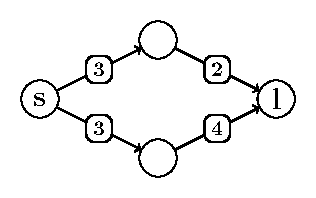
\includegraphics[scale=0.8]{Fig2.pdf} & 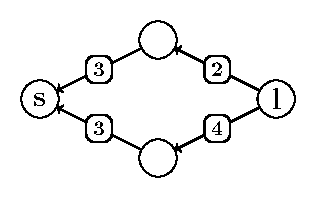
\includegraphics[scale=0.8]{Fig3.pdf}\\
 $G=(V,A)$ & $G^r=(V,A^r)$\\
\end{tabular}
\end{center}
\end{figure}

}}\end{center}

A {\bf route} $r$ is a sequence of arcs $a_0, \ldots , a_{n-1}$, with $a_i=(u_i,u_{i+1}) \in A$ such that $u_0 \in L$ and $u_n \in S$.
The {\bf latency} of a vertex $u_i$ in $r$, with $i \geq 1$, is defined by $$\lambda(u_i,r)= \sum\limits_{0 \leq k <i} Dl(a_k)$$ We also define $\lambda(u_0,r)=0$.
The latency of the route $r$ is defined by $\lambda (r)= \lambda (u_n,r)$. In graph theory, a route is a simple path in the graph, and its latency is its weight. 


A {\bf routing function}  ${\cal R}$ is an application associating a route  ${\cal R}(s,l)$ to each couple $(s,l) \in S \times L$ in $G$.
Moreover ${\cal R}$ satisfies the \emph{coherent routing} property: the intersection of two routes must be a path.

For simplicity, we assume that we have as many source nodes as we have leaves (${\cal S} = {\cal L})$.
A {\bf ${\cal R}$-matching} is a bijection $\rho :S\rightarrow L$ which associates to each $s_i \in \{s_0,...,s_{{\cal S}-1}\}$ 
a $l_i \in \{l_0,...,l_{{\cal L}-1}\}$.
A \rmatching defines a set $\{r_0, \ldots ,r_{{\cal L}-1}\}$ of ${\cal L}$ routes in ${\cal R}$ such that $\forall i\,, r_i = {\cal R}(s_i,l_i)$.

The quintuplet $N=(G,S,L,{\cal R},\rho)$ defines a \matchedgraph. We call $N^r$ the quintuplet $(G^r,S,L,{\cal R},\rho^r)$, 
where $\rho^r$ is the \rmatching obtained using the same routes, with inverted arcs.

\end{subsection}
\begin{subsection}{Slotted time Model}
In our model, the time is discrete. The unit of time is one slot. Two values are expressed in time slots : 
\begin{enumerate}
 \item the emission time of a message by a node, the {\bf message length},
 \item the time taken by a message to cross a link, the {\bf delay} of an arc).
\end{enumerate}

Let $P>0$ be an integer called {\em period}. 
A $P$-periodic affectation of N, a matched graph consists in a set  ${\cal M}=(m_0, \ldots ,m_{{\cal L}-1})$
of ${\cal L}$ integers that we call \emph{offset}. 
Each time window is divided in $P$ slots and the number $m_i$ represents the first slot number used by the route $r_i$ at its source.
We define the first time slot at which a message arrive at any vertex $v$ of the route by $$t(v,r_i) = m_i+\lambda(u,r_i) \mod P.$$

Let us call $[t(v,r_i)]_{T,P}$ the values of the time slots used by a route $r_i$ in a vertex $v$. 
Those values are forming a continuous set of values starting at $t(v,r_i) \mod P$ and ending at $t(v,r_i) + T \mod P$.
For a given instance, P and T does not change at any moment, indeed, the size of the messages is the same for any route, and the period is also the same for any vertex.
So, since P and T are fixed, we simplify the notation by $[t(v,r_i)]$.

A $P$-periodic affectation must have no {\em collision} between two routes in $\rho$, that is $\forall r_i, r_j \in \rho, i \ne j$,
we have $$[t(u,r_i)] \cap [t(u,r_j)] = \emptyset .$$

\fbox{\parbox{12cm}{
Notice that the notion of $P$-periodic affectation \textbf{is not monotone} with regard to $P$. 
Indeed, we can build a {\bf ${\cal R}$-matching} of a graph, with ${\cal L}$ routes $r_1, \dots, r_l$ which all intersect two by two and
such that if $r_i$ and $r_j$ have $v$ as first common vertex we have $\lambda(v,r_i) - \lambda(v,r_j)=1$.
Therefore there is a $2$-periodic affectation by setting all $m_i$ to $0$.

\begin{tabular}{cc}
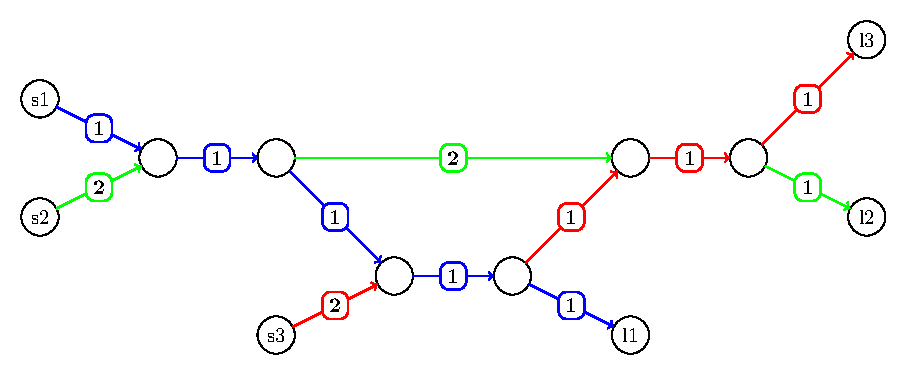
\includegraphics[scale=0.5]{Fig5.pdf} & 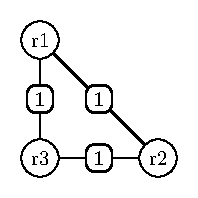
\includegraphics[scale=1]{Fig7.pdf}\\
 $\lambda(v,r_i) - \lambda(v,r_j)=1$ & Conflict graph\\
\end{tabular}\newline

On the other hand if we set all $\lambda(v,r_i) - \lambda(v,r_j)=P$, there is no $P$-peridodic affectation if $P<l$.

\begin{tabular}{cc}
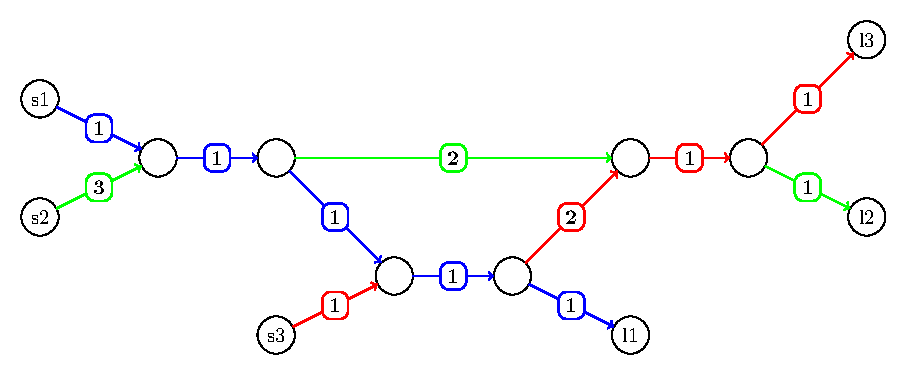
\includegraphics[scale=0.5]{Fig6.pdf} & 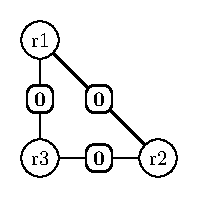
\includegraphics[scale=1]{Fig8.pdf}\\
 $\lambda(v,r_i) - \lambda(v,r_j)=2$ & Conflict graph\\
\end{tabular}\newline
\begin{center}
 Here for P=2, there is no P-Periodic affectation.
\end{center}

Therefore if we choose $P$ odd and $l=P+1$, there is no $P$-peridodic affectation but modulo $2$ all $\lambda(v,r_i) - \lambda(v,r_j)$
are equal to one thus we have a $2$-periodic affectation. 
}}
\end{subsection}
\begin{subsection}{Topology}

This project focuses on the analysis of a fronthaul network. In those kinds of networks, we can differentiate three kinds of
topologies. Each one of them correspond to a real configuration, depending of the distance between the BBU and the RRH.
\begin{enumerate}
 \item Topology 1 : A basic network topology, composed of some base stations, represented by source nodes $S$, all connected to the same switch,
which will be a vertex, connected himself to another vertex, corresponding to a switch, connected to some leave nodes $L$ representing the Antennas.
\item Topology 2 : A network containing an optical ring, such that some sources nodes may join it anywhere, not intersecting themselves before the ring,
and some set of leave nodes are also leaving at any point of the ring.
\item Topology 3 : The general case : A DAG, on which we may restrict parameters as the degree or the number of vertices to represent graphs corresponding to realistic networks.
\end{enumerate}
\fbox{\parbox{12cm}{
\begin{figure}[H]

\begin{center}
 
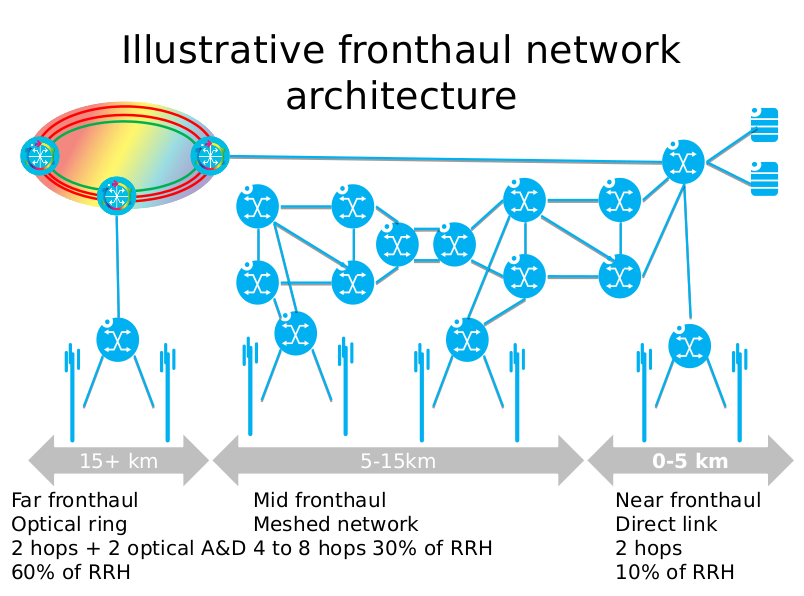
\includegraphics[scale=0.4]{fronthaul0.png}\\

\end{center}
\caption{From left to right: Topologies 2, 3 and 1 representing respectively the far, mid and near fronthaul.}
\end{figure}
}}\\

This report focus on studying the first topology, which is already reach enough to yield interesting enough questions.

\end{subsection}

\end{section}
\begin{section}{Problem}
   
The application we address here by studying the problems defined above is the following. Consider a fronthaul network in which source nodes in $S$ represent BBU,
each one able to do a remote process for RRH represented by leaves node in $L$. Consider a ${\cal R}$-matching $\rho$ of $S$ in $L$. Consider a leaf $l$, its dedicated source node $s$
and $R(l,s)$ the route from $l$ to $s$ in $R$. We consider a $P$-periodic affectation of N, and also another $P$-periodic affectation of $N^{r}$.
The periodic process is, for each route, the following one:
\begin{enumerate}
 \item During each period of duration $P$, $l$ sends a message to its source $s=\rho(l)$, using its routes according to the $P$-periodic affectation of N. 
 \item When a source $s=\rho(l)$ receive a message from $l$, it makes a computation. This computation time is fixed.
 \item After this computation time, $s$ sends a message to $l=\rho(l)$ according to the $P$-periodic affectation of $N^{r}$.
\end{enumerate}

\fbox{\parbox{11cm}{
\begin{center}
\scalebox{0.6}{
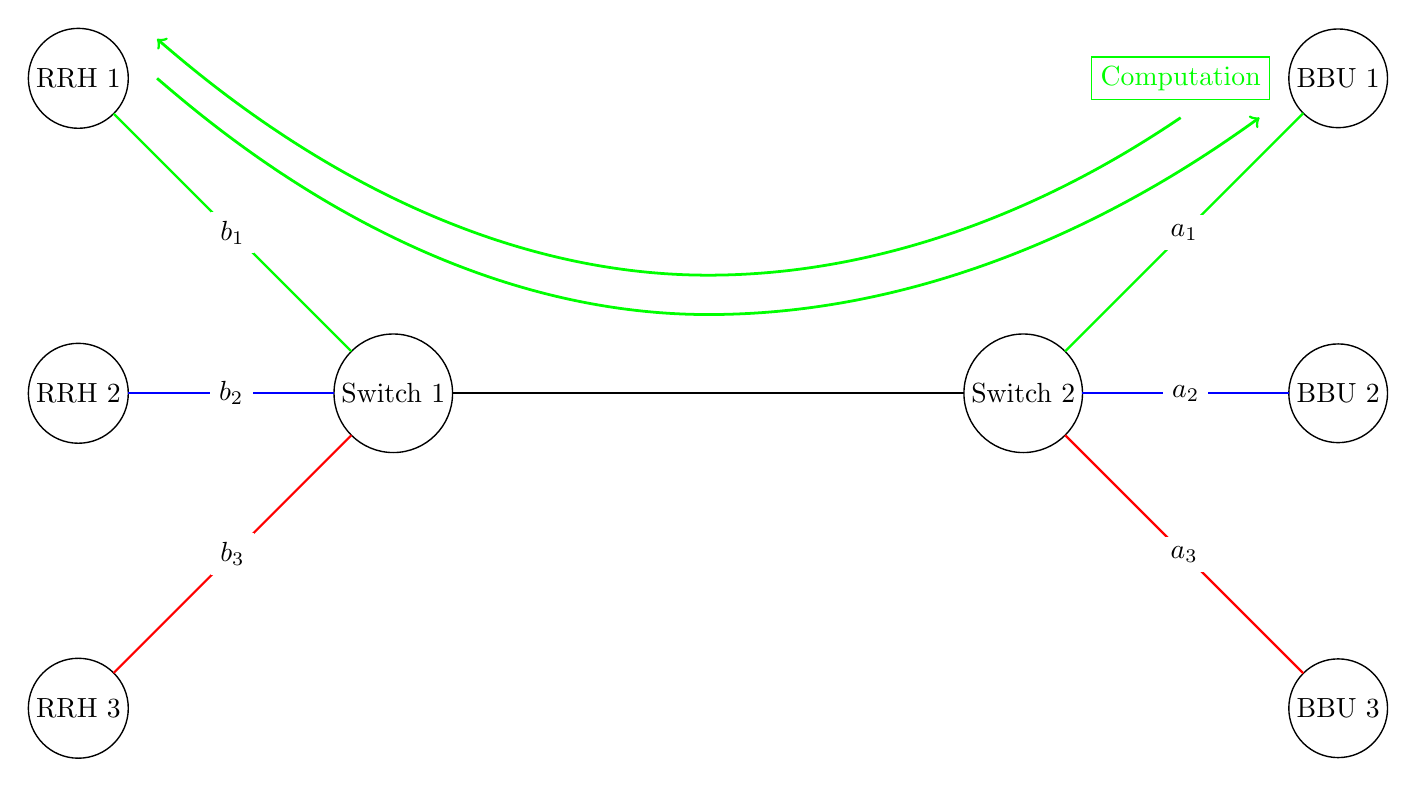
\begin{tikzpicture}
  \SetGraphUnit{5}
  \Vertex[x=0,y=0]{RRH 3}
  \Vertex[x=0,y=4]{RRH 2}
  \Vertex[x=0,y=8]{RRH 1}
  
  \Vertex[x=16,y=0]{BBU 3}
  \Vertex[x=16,y=4]{BBU 2}
  \Vertex[x=16,y=8]{BBU 1}
  
  \Vertex[x=4,y=4]{Switch 1}
  \Vertex[x=12,y=4]{Switch 2}  
  \tikzset{
  EdgeStyle/.append style = {green} }
  \Edge[label = $a_1$](BBU 1)(Switch 2)
  \Edge[label = $b_1$](Switch 1)(RRH 1)
  
  \tikzset{
  EdgeStyle/.append style = {blue} }
  \Edge[label = $a_2$](BBU 2)(Switch 2)
  \Edge[label = $b_2$](Switch 1)(RRH 2)
  
  \tikzset{
  EdgeStyle/.append style = {red} }
  \Edge[label = $a_3$](BBU 3)(Switch 2)
  \Edge[label = $b_3$](Switch 1)(RRH 3)
  
  \tikzset{
  EdgeStyle/.append style = {black} }
  \Edge(Switch 1)(Switch 2)
  
  \draw[->,line width=1pt,green] (1,8) parabola bend (8,5) (15,7.5);
  \node[draw,green] at (14,8) {Computation};
  \draw[<-,line width=1pt,green] (1,8.5) parabola bend (8,5.5) (14,7.5);


\end{tikzpicture}
}
\end{center}}}\\

On source nodes, between the end of computation time and the emission time of the message (given by the $P$-periodic affectation), there is a {\emph waiting time}. 
We define by $\omega : r \rightarrow \mathbb{N}$ the waiting time of a route $r$ in the ${\cal R}$-matching considered, i.e. the time during which the
message is ''sleeping``, waiting to be sent through the network.


We will find two P periodic affectations; one for the messages going from the RRH to the BBU, and another one for the answers going from BBU to the RRH. Those two P-periodic affectation have the same period P. 
If the messages have to be buffered, we can only do it in sources nodes.
We define by $\theta$ the computation time required at the source node before sending an answer to it's leave node.

Let us call $T (r)$ the process time on a route $r$: $$ T (r) = 2\lambda (r) + \omega (r) + \theta$$

Since $\theta$ is the same on every route, we can simplify the model by removing $\theta$. Whether we want to consider it, we only have to lengthen all 
links before source nodes by $\frac{\theta}{2}$. 


In our network application, since $P$ and the ${\cal R}-matching$ are given, we do not need to minimize $P$ because P is given.
Therefore we want to optimize the time taken by the messages to do the TwoWayTrip in order to ensure a good level of quality of service.

A {\bf TwoWayTrip affectation} of $N$ is a set of pairs $ ((m_0,x_0),...,(m_{{\cal L}-1},x_{{\cal L}-1}))$ in which ${\cal M} = (m_0,...,m_{{\cal L}-1})$ 
is a $P$-periodic affectation of $N$,${\cal X} = (x_0,...,x_{{\cal L}-1})$ is a $P$-periodic affectation of $N^r$, in which :
$$ \omega_i = x_i - (m_i + \lambda(r_i)) \mod P .$$ 

Here $\omega_i$ are the waiting times on the route $r_i$, $\omega_i = \omega(r_i)$.Since ${\cal M}$ and ${\cal X}$
are some P-periodic affectation, they must have no collisions as we defined above :
$$[t(u,r_i)] \cap [t(u,r_j)] = \emptyset .$$

% In this topology, once the first central switch passed, there is no more possible collisions between two routes, so, 
% there is an unique vertex on each matched graph N or N$^r$ on which a collision is possible.
% We can simplify the notation of  $[t(u,r_i)]$ by $[t(i)]$, where $[t(i)]$ is the interval taken by the route $r_i$
% in the conflict point of the matched graph corresponding to the P-periodic affectation.


Our real network problem is the following:\\

\noindent {\bf Problem Periodic Assignment for Low Latency(PALL)} 

\noindent {\bf Input:} matched graphs $N$, integer $P$, $ T_{max}$.

\noindent {\bf Question:} does there exist a TwoWayTrip affectation of $N$, such that $\forall r \in \rho$, $T(r) \le T_{max}$.

Once this decision problem established, we can consider two optimisation problems, derived from the previous problem in which
we try to minimise different functions of T(r).\\

\noindent {\bf Optimization goal 1:} minimizing max(T(r)).

Minimizing the longest TwoWayTrip time of all routes allows to ensure that no route will exceed the deadline of 3ms.\\

\noindent {\bf Optimization goal 2:} minimizing $\sum_{r \in \rho}  T(r)$ (equivalent to minimizing $\sum_{r \in \rho}  \omega(r)$.

By minimizing the sum of all the routes, we allow a better global Quality of Service through the network.\\
\begin{subsection}{Restrictions of topology 1}
\fbox{\parbox{12cm}{
 \begin{figure}[H]
\begin{center}

 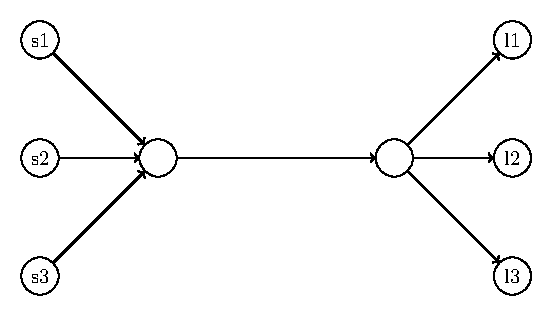
\includegraphics[scale=1]{Fig4.pdf}\\
  \caption{Example of topology 1.}
 
\end{center}
\end{figure}
}}\\


In the considered topology, there is 3 cases :
\begin{itemize}
 \item 1: When the weight of the links from source nodes are all equal. This is the closest case to the reality, and also the easier to solve.
 \item 2: When the weight of the leave nodes links are all equal .
 \item 3: When all the links have different weights.
\end{itemize}
The middle link can be represented without weight, because it is common to all the routes and have no influence of the values of T(r), so it can be simplified in computation. 

\end{subsection}
\end{section}
\begin{section}{Related Work}

The following articles helps us to approach our problem, but they all have some common limits next to our problem :
\begin{enumerate}
 \item Those articles consider the messages as one slot it their slotted time. In our situation, it is hard to represent the messages as one slot because our messages are modelled by many slots, and the messages can take many different begin offsets. In the slotted time models when one messages is represented by one slot, our problem does not find it's place.
 \item Each article helps us to have an idea how to find a P-periodic affectation, but none cover a possible TwoWayTrip. 
 \item Excluded the Circular-coloring.
 
\end{enumerate}

\begin{subsection}{Path Coloring and Call Scheduling}
Let us have a look on an article of Thomas Erlebach and Klaus Jansen about the Path coloring and Call Scheduling \cite{erlebach2001complexity}.
Those two Methods are similar to our problem.

\paragraph{Path Coloring}
The authors try to solve the scheduling of messages over optical networks. A connection between two nodes must be established, by reserving a wavelength on all links of the
path between the two nodes. The number of wavelengths is limited, so it is necessary to find a way to use the minimum number of wavelengths for a set 
of connections.

The model used is a graph $G=(V,E)$ in which the vertex represent the switches and the links are modeled by the edges. The goal is to give to each
couple of vertex (u,v), a path and a color representing the connection, such that any other couple using a common edge in its path has not the same
color than (u,v). The problem called path coloring is to minimise the number of color used.

Applied to our problem, path coloring gives a different color to each couple BBU/RRH, because they all share the same common link.
Due to our central common links, each color of the path coloring
would correspond to a message in our problem. Considering our slotted time model in which a message uses more than one slot,
we cannot reduce a part of our problem to path scheduling.

Furthermore this approach does not treat about the periodicity.


\paragraph{Call Scheduling}
In bandwidth reservation networks, the links have different bandwidth and every message 
requires a certain bandwidth reservation. The call scheduling problem problem is to set the paths and the starting times of the connection requests.
The goal is to minimise the latest completion time i.e. the moment in which all the messages are transmitted.

To solve this problem, the authors are using a graph $G=(V,E)$, in which the edges gets a capacity representing the bandwidth.
A call is represented by a couple (u,v) of vertex, a bandwidth requirement and a duration. The goal is to give a starting time to each call
such that any call has enough bandwidth on it's links when it is active.

In our problem all the bandwidth requirement, call duration and edge capacities are the same.
On the other hand, solving call scheduling does not solve our TwoWayTrip problem, since it only deals with one P-periodic affectation of the TwoWayTrip and does not take into account the periodicity.

Furthermore, this article does not give a polynomial algorithm to solve path coloring or call scheduling.

\end{subsection}

\begin{subsection}{A fast algorithm for single processor scheduling}
The article ''A fast algorithm for single processor scheduling`` \cite{simons1978fast}, by Barbara Simons presents an efficient algorithm for task 
scheduling on a single processor. All the tasks have the same execution time. The complexity of this algorithm is $O(n^2\log(n))$, n is the number of tasks.

This algorithm considers a set of tasks which have a release time and a deadline. The goal is to schedule the tasks on a single processor such
that each task does not start before its release time and stop before its deadline.
A scheduling is a set of starting times for the tasks which satisfies the previous conditions.
The algorithm finds a solution, if it exists, which minimises the time at which the last task is completed.

\paragraph{Running}
The algorithm is divided in three parts.
The main algorithm which schedule the task in a greedy way, by selecting the task according to two criteria:
\begin{enumerate}
 \item Select in the not scheduled tasks those whose release time is lower than the actual clock.
 \item Between those eligible tasks, select the one that has the lower deadline.
\end{enumerate}

When a task is selected, put it in the scheduling and update the clock of the duration of the tasks.
If the deadline of the selected task is lower than the new clock, then this is a crisis task.
When a crisis occurs, call the first subroutine : the {\bf CRISIS} subroutine.

Let us call X the crisis task.
The crisis subroutine select between the scheduled tasks the one that have been scheduled the last, and that have an higher deadline than the crisis task.
If such a task exists, this task is called PULL(X). If not, the algorithm fails.
All tasks scheduled after PULL(X) are placed in a new set called ''restricted set``.
Pull(X) does not belong to the r.s. but X does.

Once this r.s. is established, the main algorithm is applied to schedule the tasks. If a crisis occurs, call the crisis subroutine on the new tasks.
If a r.s. contains others inner r.s. do not reschedule the tasks in those inner restricted sets. Consequently, the main routine schedule 
the tasks by interval. In case of the new schedule overlaps an inner r.s. call the third subroutine, {\bf INVADE}.

The invade subroutine reschedule the r.s.from the new beginning date which is the deadline of the last scheduled task. If a crisis or an invade occurs,
call the appropriate subroutine.

\paragraph{Adaptation to our problem}
This algorithm helps us to solve problem of finding the second P-periodic affectation of the TwoWayTrip, when the first is fixed. 
The tasks are the message transiting from the BBUs to the RRHs, the release times are the time on which the message will be able to be sent,
and the deadlines are determined according to the 3ms max of the TwoWayTrip.

To take care about the periodicity, we just have to adjust the deadline of the tasks such that there is no tasks with a deadline 
higher than the fixed period.

\end{subsection}

 At the beginning of the internship, we tried to solve the global problem (topology 3). We started to work on conflict graphs, representing
 the collision between two routes. The vertices of a conflict graph $G = (V,E)$ are the routes, and there is an edge between two vertices
 if and only if there is a common arc between the two routes in the matched graph.
 
\begin{subsection}{T-coloring}


 We first looked at an article written by Rafl Borndöfer, Andreas Eisenblätter, Martin Grotschel and Alexander Martin, Frequency assignment
 in cellular Phone Networks \cite{borndorfer1998frequency}. The authors of this articles use the T-Coloring to assign some channels to some 
 transceivers antennas in radio networks. There is a few channels and a lots of transceivers, the goal is to give a channel to each transceivers
 such that the number of interferences in the network is as low as possible.
 
 The T-coloring is the labelling $f$ of the vertices in a graph G=(V,E), given a set of integers T, $0 \in$ T, such that 
 $|f(v) - f(w)| \notin T$.
 The authors use this approach to label their graph using a different set T for each vertex of the graph.
 In the case of a conflict graph coloration, the set of forbidden values is a single element, so the approach is too general.

\end{subsection}
\begin{subsection}{Circular coloring}

 The circular coloring ,studied by Xuding Zhu\cite{zhu2006recent}\cite{zhu2001circular} and Bing Zhou\cite{zhou2013multiple},
 is a coloring approach with real numbers instead of integers. The goal is to give to each vertex of a graph 
 a real interval of a circle such that no adjacent vertex has a common interval on the circle. This is a little variation of a
 basic coloring, but in this case, it just consider classic graphs, meanwhile the conflict graphs we need to color have some weight
 on the edges. Therefore, the circular coloring is not adapted to our model.

\end{subsection}

\begin{subsection}{Complexity results on the topology 3}
 Dominique Barth, Yann Strozecki, Christian Cadéré and Olivier Marcé from the laboratory David and Nokia Bell Labs France started to study the complexity for the topology 3.
 They used the conflict graph defined above to prove that it is Np-hard to solve the problem of finding a P-Periodic affectation in a model where the
 messages are only one time slot. As well, since we have a more complex model for this topology, finding the TwoWayTrip affectation
 that is composed of a P-periodic affectation is also Np-Hard. However, we did not prove that it is Np-Hard to find
 a TwoWayTrip on the first topology.
\end{subsection}

 \end{section}

Despite the research we made on the subject, we did not find a previous study treating about this process containing two 
following affectations.
\end{chapter}

\begin{chapter}{Algorithms}

In this chapter, one can find the different algorithms imagined to solve the problem. We present each algorithm, their property and their complexity.
Except for the LSO, Yann and I have imagined and developed all the algorithms.

\begin{section}{Solution without waiting times}

Firstly, let us consider the first case of the topology 1 defined above, where all the links going to the BBU
have a weight of 0. It is the easiest to solve. 
Indeed, if we schedule all messages following each others, we will obtain an optimal
$T_{max}$ : there is no waiting times on any route.
Also, all the message will cross the first switch, without collisions, then 
they will not be another conflict point between all routes.
Indeed, there is only two collision points on the topology 1, the two switches.
Here, according to the null weight on the links between the sources switch and the BBU,
there is no shift between the different routes on the graph after the first switch.
So the scheduling in the first switch will be the same in the second switch,
and the messages will not conflict again.\\
 
 \fbox{\parbox{11cm}{
 \scalebox{0.6}{
 \begin{tikzpicture}
   \SetGraphUnit{5}
   \Vertex[x=0,y=0]{RRH 3}
   \Vertex[x=0,y=4]{RRH 2}
   \Vertex[x=0,y=8]{RRH 1}
   
   \Vertex[x=16,y=0]{BBU 3}
   \Vertex[x=16,y=4]{BBU 2}
   \Vertex[x=16,y=8]{BBU 1}
   
   \Vertex[x=4,y=4]{Switch 1}
   \Vertex[x=12,y=4]{Switch 2}  
   \tikzset{
   EdgeStyle/.append style = {green} }
   \Edge[label = 0](BBU 1)(Switch 2)
   \Edge[label = $b_1$](Switch 1)(RRH 1)
   
   \tikzset{
   EdgeStyle/.append style = {blue} }
   \Edge[label = 0](BBU 2)(Switch 2)
   \Edge[label = $b_2$](Switch 1)(RRH 2)
   
   \tikzset{
   EdgeStyle/.append style = {red} }
   \Edge[label = 0](BBU 3)(Switch 2)
   \Edge[label = $b_3$](Switch 1)(RRH 3)
   
   \tikzset{
   EdgeStyle/.append style = {black} }
   \Edge(Switch 1)(Switch 2)
 
   \node (0) at (1,-1){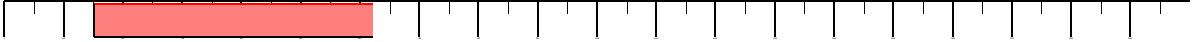
\includegraphics[scale=0.1]{chronogrames/4.jpeg}};
   \node (1) at (1,3){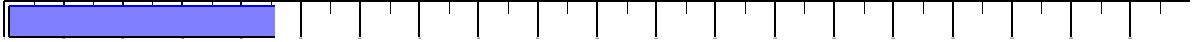
\includegraphics[scale=0.1]{chronogrames/1.jpeg}};
   \node (2) at (1,7){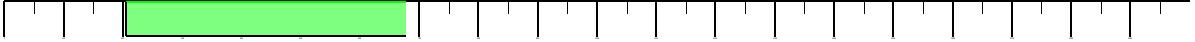
\includegraphics[scale=0.1]{chronogrames/5.jpeg}};
   \node (2) at (4,5){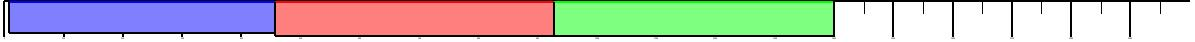
\includegraphics[scale=0.1]{chronogrames/6.jpeg}};
 \end{tikzpicture}
 }}}\\

This solution is optimal because the messages will not wait on source nodes, that is $\omega(r) = 0$, $\forall r \in \rho$. $T_{max}$ is
equal to twice the physical delay of the longest route, which is given in the input.\\


Following this observation, one can try to solve another problem for cases 2 and 3: is it possible to find a TwoWayTrip
with all $w_i = 0$ ? 

It is always possible when the windows $P$ is large enough(for example: send all messages one by one, waiting the previous one to be back),
therefore the problem is to find the smallest windows such that it is possible.

\begin{subsection}{Star affectation}
 
Let us define a simplification of a matched graph. Ignore weights on arcs starting from leaves, and the middle link.
We obtain a graph in which we have a central node, and different routes going to each sources.
Such a graph is called a \emph{star}. A star is a non-oriented graph in which each edge between the central node $C$ and each source node $s_i$
has a weight $a_i$ (corresponding to the weight of the arc in $N$), where i is the number of the route in $\rho$. The ${\cal R}$-matching $\rho$ is now
associating a route $r_i$ to a source node $s_i$.\\

\fbox{\parbox{11cm}{

\begin{center}

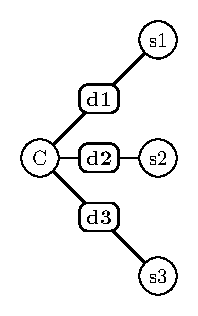
\includegraphics[scale=0.7]{Fig11.pdf}\\
Example of a star for a matched graph with 3 routes
\end{center}


}}\\


We can do this simplification of a matched graph N only if we search an affectation without waiting times : in this case, any solution
will be optimal, because the $T_{max}$ will be twice the delay of the longest route. So, a solution for a star, is a solution for a matched
graph, without waiting times. If waiting times are allowed, we are forced to consider the delay of the routes and this model is not
correct anymore.

A \emph{star affectation} is a TwoWayTrip affectation of the corresponding matched-graph $N$
in which there is no waiting time,$\omega(r) = 0 \,\forall\, r \,\in\, \rho$. 

In this simplified model, we have one parameter left: the travel time of each routes $2a_i$.
We have to set the beginning offsets $o_i$ such that a route may have collisions with the others, 
according to the definition of the collisions, given in part 2.1.2.


We define a new problem : 


\noindent {\bf Star affectation (SA)} 

\noindent {\bf Input:} a star s, integer $P$.

\noindent {\bf Question:} does there exist a star affectation of s in a period P.\\

This is our main problem, but by finding the smallest P for which there is a star affectation, we can know 
the minimal period given by our algorithm. The smallest the period is, the better is the algorithm.


\noindent {\bf Optimization :} minimizing P .\\

In the case where we find a star affectation, it gives us an optimal solution for cases 2 and 3.
In the case where there is no solution without waiting times, there still can exist some solution with waiting times in 
a period P.
\end{subsection}
\begin{subsection}{Shortest-Longest}
 
We suggest the following algorithm to find a star affectation in which $d_0$ is the shortest route, and $d_{l-1}$ the longest one, 
l is the number of routes and T is the size of the messages :

\begin{algorithm}[H]
\caption{Star affectation from shortest to longest}
\begin{algorithmic}

\REQUIRE star s
\ENSURE star affectation in $P \le l*T + 2d_{l-1} - 2d_0$
\STATE $offset \leftarrow 0$
\FORALL{routes i in $\rho$ from the shortest to the longest }
\STATE $o_i \leftarrow offset$
\STATE $offset \leftarrow offset+T$
\ENDFOR

\end{algorithmic}
\end{algorithm}

\paragraph{Running}

The message using the shortest route is sent before the others, so it come back to the central node before the others.
Recursively, the second message is sent before the others, and also will be back before the other messages. 
Because the second message is sent T slots after the first message ($o_2 = o_1 + T$, where T is the size of the message), it come back after
the end of the message one : $o_1+ T + 2a_1 \le o_2 + 2a_2$ with $a_2 \ge a_1$.

\paragraph{Period}
The period given by this algorithm is P = 2$\lambda(r_{{\cal L}-1}$) + ${\cal L}$ * T - 2$\lambda(r_0)$, if routes $\{r_0,...,r_{{\cal L}-1}\}$ are ordered
from the shortest to the longest. 2$\lambda(r_0)$ is the first slot in which the first message is starting to pass through the sources switch,
and 2$\lambda(r_{{\cal L}-1})$ + ${\cal L}$ * T  is the time at which the last message has totally passed the switch.
Therefore, the period only depends of the difference between the longest and the shortest route : the larger this value is, the larger
the period is.

\paragraph{Complexity}
This algorithm runs in $O(l.\log(l))$. It represent the cost to sort the routes.
Indeed,once the routes have been sorted,the algorithm does a constant number of instruction for each route.
\end{subsection}

\begin{subsection}{Greedy Prime}

The following algorithm is a way to find a star affectation by a greedy way.

\begin{algorithm}[H]
\caption{Greedy Prime assignment}
\begin{algorithmic}
\REQUIRE star s, window size $P$
\ENSURE star affectation in a period $\leq P$ 
\STATE $P1[P]$ slots in first way period.
\STATE $P2[P]$ slots in back way period.
\FORALL{route i in $\rho$ }

\FORALL{slot j in P1}

\IF{$[j,j+T]_P$ is free in P1}

\IF{$[j + 2d_j,j + 2d_j+T]_P$ is free in P2}

\STATE $o_i \leftarrow j$
\ENDIF

\ENDIF
\IF{No intervals are found for i}
\STATE return FAILURE
\ENDIF
\ENDFOR

\ENDFOR

\end{algorithmic}
\end{algorithm}


In this algorithm,for each route i, search for the first free slot [j,j+T] in P1 such that the slot $[j + 2d_i,j + 2d_i+T]$ in P2 is free too,
then give the route the offset j shifted by the distance from the leave to the first node.\\
This algorithm has no theoretical certitudes, but it could be in fact more efficient than greedy star assignment.


\paragraph{Complexity}
This algorithm runs in $O(n*P)$, where n is the number of routes. For each route, the algorithm tries the P possible
starting slots and tests whether there is a collision on the way back.
\todo{dire que c'est facile de tester si il y a des colisions car les messages ont la meme taille}

\end{subsection}




\begin{subsection}{Greedy Star}
 

We can also use a greedy algorithm, choosing the offset of each packet in turn so that there is no collision. 
We must chose an offset $o_i$ for each route $r_i$, so that no two routes have a collision when they return to central node.  
We denote by $[o_i]_P$ the set of times $\{ t \mod P \mid o_i \geq t < o_i + T \}$ which are the time used by the route $r_i$ on the central
link on its first use. There are no collision if for all $i\neq j$
 $[o_i]_P \cap [o_j]_P = \emptyset$. Moreover no two routes must have a collision on the way back, hence we must have for all $i\neq j$
 $[o_i + a_i]_P \cap [o_j + a_j]_P = \emptyset$.
 
 

\begin{algorithm}[H]
\caption{Greedy star assignment algorithm}
\begin{algorithmic}
\REQUIRE star s, window size $P$
\ENSURE star affectation in a period $\leq $ P 
\STATE $P1[P/2T]$ slots in first way period.
\STATE $P2[P/T]$ slots in back way period.
\FORALL{route i in $\rho$ }

\FORALL{slot j in P1}

\IF{P1[j] is free}

\STATE shift $\leftarrow$ T- 2$d_i \mod P$ 

\IF{P2[shift + 2Tj] is free}

\STATE $o_i \leftarrow 2Tj + shift$
\ENDIF

\ENDIF

\IF{No intervals are found for i}
\STATE return FAILURE
\ENDIF
\ENDFOR

\ENDFOR

\end{algorithmic}
\end{algorithm}



\paragraph{Running}
In this algorithm,for each route, search for a free bucket in P1,then set $o_i \in [cT,cT+1]$ so that $o_i + a_i \mod P = dT$.
If $[dT,(d+1)T]$ is free, and allow the route to use the bucket $[cT,cT+1]$ at the first use of middle link.\\


\paragraph{Period}
One can prove that if $P$ is large enough with regard to $l$ and $T$, then there is always a TwoWayTrip
with waiting time $0$ with this algorithm.
 Assume $P \geq 4lT$, the algorithm works as follows. 
We cut the time windows of size $P$ into $2l$ slots of size $2T$ and we will asign one to each route.
A different slot is assigned to each route, where the offset is chosen inside the slot so that 
no collision on the first go in the central link is possible. If the slot chosen for the route $r_i$ is $[cT,(c+2)T]$,
then we set $o_i \in [cT,cT+1]$ so that $o_i + a_i \mod P = dT$. Assume that the offset of the first $i-1$ routes have been 
chosen in the previous way so that there is no collision. Since we have $P \geq 4lT$, we have at least $2l-i$ possible choices of offset without collision on the first use of the central link. Each of these choices uses a time slot of size $T$ on the way back on the central link. Since there are $i$ time slots used, and $i \leq l$, we have strictly more than $l$ possible choices and less than $l$ of them are forbidden, therefore there is a choice of offset with no collision. 
Since the algorithm works for all $i \leq l$, it finds a TwoWayTrip with waiting times $0$. 

\paragraph{Complexity}
This algorithm runs in $O(n x \frac{P}{2T})$, where n is the number of routes. For each routes, it tries the $\frac{P}{2T}$ buckets in
the first period to find an interval in the second period that does not collide with the other routes. In the worst case, the 
algorithm will browse the $\frac{P}{2T}$ slots before failing.
\todo{meme algo qu'avant sauf qu'on ne considere que les buckets}
\end{subsection}


\begin{subsection}{Exhaustive Generation}
 To try finding a solution without waiting times, we tried to implement a naive algorithm testing all the different starting offsets.
 Such an algorithm was just too slow: indeed the number of possible instances is exponential. With a period of 20000 slots,
 and 7 routes, we have over $10^{28}$ possibilities which is not practically computable.
 The following algorithm is a ''smart bruteforce``, an exhaustive generation of the possibilities with heuristics.
 
\begin{algorithm}[H]
\caption{Bruteforce}
\begin{algorithmic}
\REQUIRE Matched graph N, window size $P$, packet size T
\ENSURE 2way Trip affectation in P
\STATE BUDGET $\leftarrow$ P - l * T
\STATE offset $\leftarrow$ 0
\FORALL{route i in $\rho$ }
\FORALL{j from offset to offset + BUDGET }
\IF{Message of the route i does not collides with other routes, and some conditions are observed}
\STATE Give i the offset j
\STATE BUDGET $\leftarrow$ BUDGET - (j - offset)
\STATE offset $\leftarrow$ j
\STATE call bruteforce on remaining routes
\ENDIF
\ENDFOR
\ENDFOR


\end{algorithmic}
\end{algorithm}n

\paragraph{Running} This algorithm enumerates all the solutions by traversing a tree. The leaves of the tree are 
the TwoWayTrips without waiting times, and the nodes are partial solutions. A partial solution is choice of a starting time for a subset of the routes.
Give to the first route the first available starting offset, and then give the second route the first available starting offset etc...
\todo{parler d'une boucle}
If an offset is not compatible for a route (collisions with other routes), then try the following offset. In no offsets are available for a route,
try the next free route without starting time.
If nothing works, we backtrack \todo{expliquer backtrack}.

We have implemented cuts so the algorithm avoid to browse some parts of the tree that will not give any solution.
\begin{enumerate}
 \item The budget : It is the number of slots that can be waste in the period. If this budget comes below 0, then the period is too small with regard to
 the solution.
 \item When a starting offset is given to a route, the interval used by the route on the source's switch is also set. If there is less than T slots
 between the end of the previous message and the beginning of the actual message, then no future messages can be scheduled in this gap.
 So, if the solution isn't found with the first offset, the algorithm will directly skip to the offset corresponding to a gap of T slots.
 \item There is also a budget for the second period. If too much slots are lost between two messages, the algorithm will skip the partial solution.\todo{etre plus precis}
\end{enumerate}

Because of the cuts,one can hope that this algorithm which have an exponential complexity works fast enough to find some solution in our problem.

\end{subsection}

 \end{section}

\begin{section}{Finding a TwoWayTrip with waiting times}
\begin{subsection}{Waiting times are useful}
 
The following example shows us that you can find a TwoWayTrip affectation such that there is no waiting time, but it needs a greater time window P than a
solution with waiting times.

Consider the graph : 
\begin{center}
 
\fbox{\parbox{11cm}{  
\scalebox{0.6}{
\begin{tikzpicture}
  \SetGraphUnit{5}
  \Vertex[x=0,y=0]{l1}
  \Vertex[x=0,y=4]{l2}

  
  \Vertex[x=16,y=0]{s1}
  \Vertex[x=16,y=4]{s2}

  \Vertex[x=4,y=2]{Switch 1}
  \Vertex[x=12,y=2]{Switch 2}
  

  \tikzset{
  EdgeStyle/.append style = {red} }
  \Edge[label = 1](s1)(Switch 2)
  \Edge[label = 10](Switch 1)(l1)
  
  \tikzset{
  EdgeStyle/.append style = {green} }
  \Edge[label = 10](s2)(Switch 2)
  \Edge[label = 1](Switch 1)(l2)
  
  
  \tikzset{
  EdgeStyle/.append style = {black} }
  \Edge(Switch 1)(Switch 2)
\end{tikzpicture}
  }}}\\
\end{center}

Consider messages of 10 slots. If you search for a P-periodic affectation, without using waiting times, there are 2 choices : 
\begin{itemize}
 \item l1 is sent before l2 : the message from l1 will leave A after 11 slots.X is he minimal time slot in which l2 can emit. 
 To avoid collisions with the message from l1 in A,l2 must emit after 1 slot :  $X\ge1$.
 In the other way, the message from l1 will use B from time slot 21 to 30. The route from l2 is 12 units long from l2 to B. So, to avoid collisions with 
 the message from l1 in B $X+12 \ge 31 \rightarrow x\ge 19$. Then, by taking $X=19$, the time
 windows is at least 38 slots in A (corresponding to the transit time of the 2 messages and the time lost between those 2 transits).
 \item l2 is sent before l1: symmetrically the collision the collision occurs in node A if l1 emits before time 19. The time window in B is at least 38 too.
\end{itemize}

\fbox{\parbox{11cm}{
\scalebox{0.6}{
  
\begin{tikzpicture}
  \SetGraphUnit{5}

  
  \node (0) at (1,-1){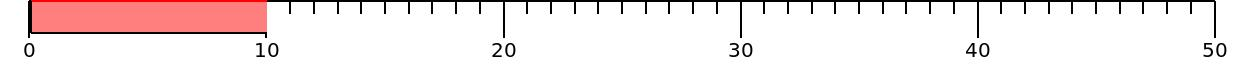
\includegraphics[scale=0.1]{chronogrames/10.jpeg}};
  \node (1) at (1,5){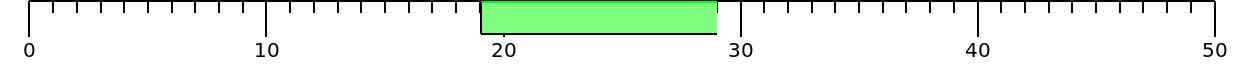
\includegraphics[scale=0.1]{chronogrames/11.jpeg}};
  \node (2) at (5,2){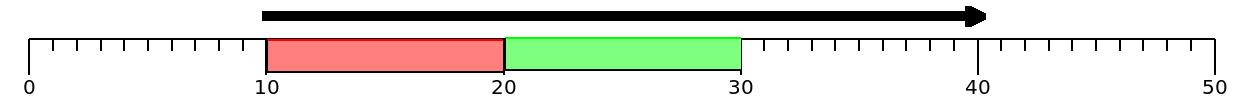
\includegraphics[scale=0.1]{chronogrames/12.jpeg}};
  \node (3) at (10,2){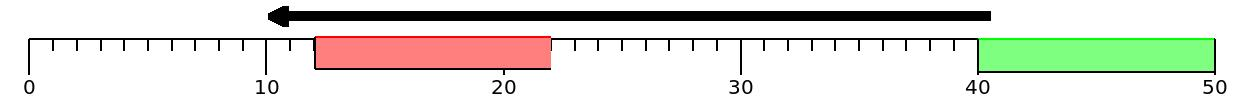
\includegraphics[scale=0.1]{chronogrames/15.jpeg}};
  \node (4) at (15,-1){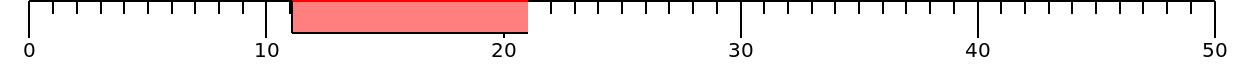
\includegraphics[scale=0.1]{chronogrames/13.jpeg}};
  \node (5) at (15,5){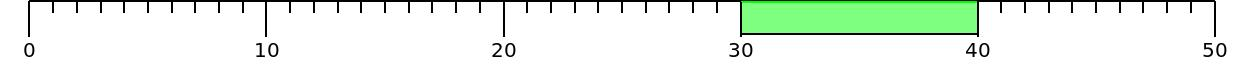
\includegraphics[scale=0.1]{chronogrames/14.jpeg}};
  
     \Edge(2)(3)
    \tikzset{
    EdgeStyle/.append style = {red} }
    \Edge[label = 10](0)(2) 
    \Edge[label = 1](3)(4)

    \tikzset{
    EdgeStyle/.append style = {green} }
    \Edge[label = 1](1)(2)
    \Edge[label = 10](3)(5)
\end{tikzpicture}
  } 
  Without waiting times: Window of 38(2k + 18) slots, $T_{max}$ = 22 slots.
  }}\\
 


If we allow waiting times: there is an easy scheduling using only a 3 time slots windows : 
Sending message 1 at time 0, message 2 at time 1, so the messages will not cross A in the same time. to be sent back,
message 2 comes back immediately and is using B from slots 13 to 22,then message 1 is using B from slots 23 to 32, waiting 2 time slots at s1.

So the smaller time windows is 20, half smaller than best solution without waiting times.\\

\fbox{\parbox{11cm}{
 \scalebox{0.6}{
  \begin{tikzpicture}
  \SetGraphUnit{5}

  
  \node (0) at (1,-1){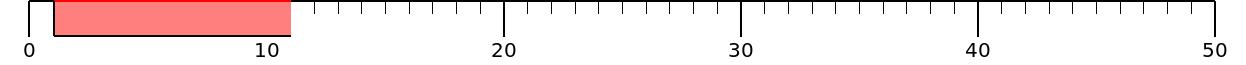
\includegraphics[scale=0.1]{chronogrames/22.jpeg}};
  \node (1) at (1,5){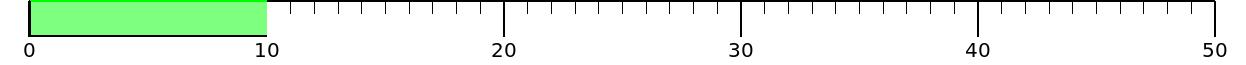
\includegraphics[scale=0.1]{chronogrames/21.jpeg}};
  \node (2) at (5,2){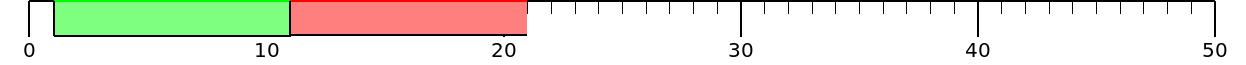
\includegraphics[scale=0.1]{chronogrames/23.jpeg}};
  \node (3) at (10,2){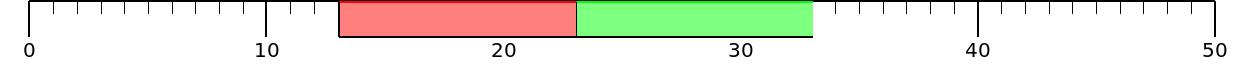
\includegraphics[scale=0.1]{chronogrames/26.jpeg}};
  \node (4) at (15,-1){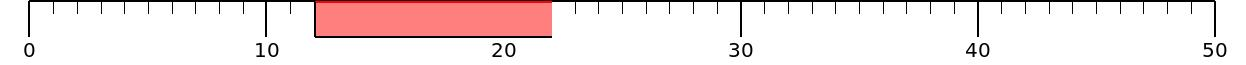
\includegraphics[scale=0.1]{chronogrames/25.jpeg}};
  \node (5) at (15,5){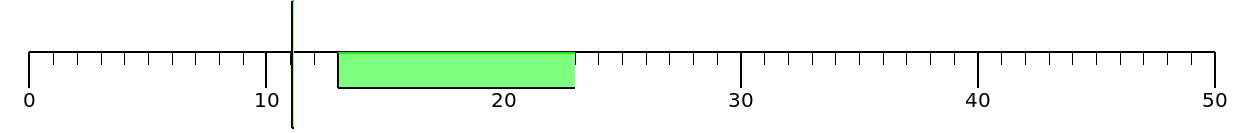
\includegraphics[scale=0.1]{chronogrames/24.jpeg}};
  
     \Edge(2)(3)
    \tikzset{
    EdgeStyle/.append style = {red} }
    \Edge[label = 10](0)(2) 
    \Edge[label = 1](3)(4)

    \tikzset{
    EdgeStyle/.append style = {green} }
    \Edge[label = 1](1)(2)
    \Edge[label = 10](3)(5)
\end{tikzpicture}
  }
  
    With waiting times: Window of 20(2k) slots, $T_{max}$ = 24 slots.

  }}\\
  
  Allowing the waiting times gave us the possibility to reduce the period from 38 slots to 20, with only 2 times slots added to $T_{max}$.
\end{subsection}
\begin{subsection}{Main algorithm : Longest-Shortest}
 

To find a solution allowing waiting times, the following heuristic is suggested :

\paragraph{Running}
\begin{itemize}
 \item 1 On leaves node, the messages are scheduled so that they are following each others, from the longest route to the shortest route.
 \item 2 On sources node, let the message able to come back first pass.
 \item 3 Once this message has passed, look at all the eligibles message able to be back at the sources node during the transit of the previous one.
 \item 4 Let the eligible message on the longest route transit in the node first after the previous one, possibly delayed by a little waiting time to avoid crossing.
 \item 5 delay the others with a waiting time.
 \item 6 while all the messages are not scheduled, get back to 3
\end{itemize}

\begin{algorithm}[H]
\caption{Longest shortest with waiting times}
\begin{algorithmic}
\REQUIRE Matched graph N, window size $P$, packet size T
\ENSURE 2way Trip affectation in P
\STATE offset $\leftarrow$ 0
\FORALL{route i in $\rho$ from the longest to the shortest }
\STATE  $m_i \leftarrow$ offset
\STATE offset $\leftarrow$ offset + T
\ENDFOR
\STATE offset $\leftarrow$ 0
\STATE take i such that $r_i$ is the first route to come back in sources node
\STATE $w_i \leftarrow $ offset;
\STATE offset $\leftarrow$ $a_i$ + T
\WHILE{there is a route which has no $w_i$}
\STATE take i such that $r_i$ is the eligible route.
\STATE $w_i \leftarrow $ offset - $a_i$;
\STATE offset $\leftarrow$ offset + T

\ENDWHILE

\end{algorithmic}
\end{algorithm}


\paragraph{Period}
This algorithm gives us solution with the minimum possible period: ${\cal L}$ x T. Indeed, all the messages are scheduled following each others on switches:
there is no wasted time between the transit of two messages.

\paragraph{Analysis}
For the case 1, this algorithm is similar to the obvious way to schedule the messages mentioned above. It gives optimal solution without increasing 
the computation time.

For the case 2, this algorithm gives optimal solutions: Indeed, in the manner we order messages, from leaves toward sources,
the messages are sent from the one using the longest route to the one using the shortest one. Number the routes in this order from 1 to ${\cal L}$.

We have $\forall \ i<j$, $r_i<r_j$.
The first message leaves the source switch at time 2$r_1+T$, the second message, can use it at the time 2$r_2+T$.
The second message waited $2r_1+T-(2r_2+T) = 2(r_1-r_2)$ to use the middle link. So, the second message leave the source switch at time
2$r_2+T + 2(r_1-r_2) = 2r_1 +T$.
By induction, all messages will take $2r_1 +T$ slots for the TwoWayTrip.
Consequently, for this case, the heuristic is optimal, because the longer route has no waiting time and no TwoWayTrip is longer than the longer route one.

We have no theoretical values for the case 3. The experimental study is in the following chapter.
\todo{on pense que ca ne donne sans doute pas la solution optimale, mais que sur certains parametres dans la prochaine partie ca marche bien}

\paragraph{Complexity}
By using a binary heap to implement a priority queue, this algorithm runs in O(n.log(n)), 
where n is the number of routes. For each route, there is a deletion and an insertion in the heap.
\end{subsection}

\begin{subsection}{Barbara Simons's Algorithm}
 The algorithm studied by Barbara Simons's article \cite{simons1978fast} gives us an improvement of the longest-shortest algorithm.
 \begin{algorithm}[H]
\caption{Simons Main Algorithm}
\begin{algorithmic}
\REQUIRE Set of tasks S
\ENSURE Scheduling in a minimal time.
\STATE CLOCK $\leftarrow$ 0
\WHILE{ S $\ne \emptyset$}
\STATE Select X the not scheduled job with the lower deadline in the eligible jobs
\IF{X has a CRISIS}
\STATE call CRISIS(X)
\STATE CLOCK = end of the returned r.s.
\ELSE
\STATE CLOCK += task-length
\ENDIF

\ENDWHILE

\end{algorithmic}
\end{algorithm}
As a reminder, a job is eligible if its release date is lower or equal to the actual clock. If no such a job exists, the eligible job is the one
with the lowest release time.

 \begin{algorithm}[H]
\caption{Crisis Subroutine}
\begin{algorithmic}
\REQUIRE A crisis job X
\ENSURE New scheduled r.s.
\STATE backtrack over the scheduling and find PULL(X)
\IF{ PULL(x) $= \emptyset$}
\STATE Exit Failure
\ENDIF 
\STATE Remove and count the jobs in each interval between the inner restricted sets
\STATE Increase the initial interval number by 1
\WHILE{Some jobs have not been scheduled}
\STATE Use the naive algorithm to schedule the required number of jobs in each interval.
\IF{Some job X has a CRISIS}
\STATE Call CRISIS(X)
\ELSE
\IF{Some job Y invades the following r.s. S'}
\STATE call INVASION(S', $t_{S'}$)
\ENDIF
\ENDIF
\ENDWHILE

\end{algorithmic}
\end{algorithm}
$t_{S'}$ is the time at which the job Y is completed.


 \begin{algorithm}[H]
\caption{INVASION Subroutine}
\begin{algorithmic}
\REQUIRE S' a r.s., $t_{S'}$ a begin date.
\ENSURE New scheduled r.s.
\STATE Remove and count the jobs in each interval between the inner restricted sets
\WHILE{Some jobs have not been scheduled}
\STATE Use the naive algorithm to schedule the required number of jobs in each interval.
\IF{Some job X has a CRISIS}
\STATE Call CRISIS(X)
\ELSE
\IF{Some job Y invades the following r.s. S'}
\STATE call INVADE(S', $t_{S'}$)
\ENDIF
\ENDIF
\ENDWHILE

\end{algorithmic}
\end{algorithm}

\paragraph{Running}
A job $A$ has a release time $r_A$, a deadline $d_A$, and a schedule time $t_A$. The jobs have the same running time $p$.
The running of this algorithm is the following one:
The main algorithm starts to schedule the jobs by the following rules :
\begin{enumerate}
 \item To be eligible, a job needs to have a release time lower or equal to the current clock.
 \item Between the eligible jobs, schedule first the one which has the lowest deadline; Give this job the time $t_A = CLOCK$
 \item Update the clock at the time in which the scheduled task is over.
\end{enumerate}

If a selected job (let us call it X) has an insufficient time to run ($t_A + p > d_A$), then X is a CRISIS job.

The Crisis subroutine is called when there is a crisis job. It search through the schedule starting at the end,
and try to find a job with an highest deadline.
If such a job exists, it is called PULL(X). Otherwise, the algorithm fails.
Let us call PULL(X) A.
All the browsed tasks from X(included) to A(excluded) are forming a new set called restricted set S(A,X].
The algorithm tries to reschedule the jobs in S(A,X] by the main algorithm rules, if another crisis occurs, the crisis subroutine Recursively calls
itself.

In case of the crisis subroutine is backtracking over a restricted set, it does not reschedule this r.s.. The subroutine only count
the number of jobs between the r.s. and reschedule exactly the same number of jobs after the backtracking.

During this rescheduling, some jobs may overlap an r.s.. In this situation, the subroutine INVASION is called on this r.s..

The Invasion subroutine just count the number of jobs between the intervals of the r.s. and reschedule the jobs with the new starting time,
which correspond to the completion time of the task before the r.s..



\paragraph{Complexity}
This Algorithm runs in $O(n^2 \log(n))$, where n is the number of tasks. This complexity is given by the author of the article.

\paragraph{Adaptation}
This algorithm allows us to improve the second P-Periodic affectation of the longest-shortest algorithm. 
Indeed, it yield, in polynomial time, an optimal solution with a given set of jobs with release times and deadline. 
\todo{aller fixé, donc on a des release time, l'algo nous donne la meilleur maniere de faire les retours}
Because we arbitrarily chose the first P-periodic affectation, the problem is not solved.
To adapt this algorithm in the second part of the longest-shortest, we set the release time of jobs by using the longest-shortest algorithm for
the first P-periodic affectation, then we set the deadline by choosing the minimum between two values : 
\begin{enumerate}
 \item The time in which the first route came back on its sources + P-T.
 \item The maximum delay allowed - the physical transit time of the route.
\end{enumerate}
\todo{regarder si en prenant le temps des routes modulo P c'est vrai ou pas}

The first value ensure us to have a periodic process of period P. The second correspond to the first constraint of the problem : to not exceed a deadline.

\paragraph{Limitations}
Once this adaptation done, we realised that this algorithm is not efficient in our problem. Indeed, once the first P-Periodic affectation is chosen
by the algorithm, we have a set of tasks with release times and deadlines that does not trigger any crisis.
THe release times and deadlines are regularly spaced in the time (ex : (1400-7000), (3900,9500), (9000,15000) ...).
The algorithm will so take the tasks by their arrival order and send it back in the same order. If, however a crisis occurs, no tasks could be the PULL
of another one. A task can be the pull of another if it has an earlier deadline and a greater deadline, with this configuration, such a task does not exists.

\paragraph{Inference}
So, the Simons algorithm gives us the same results than the longest shortest, but it can fail if the routes are too long.
Even if the Simons algorithm is ensuring optimal solutions for a given set of tasks, it is giving the same solutions than the longest shortest, but
has a risk of failure. We will prefer the longest shortest algorithm.



\end{subsection}

\end{section}

\end{chapter}

\begin{chapter}{Performance Evaluations}

In this chapter, we will try the previous algorithm on some instances of the topology 1.

\begin{section}{Real values}
 During all the chapter, we will introduce some simulations results obtained on values corresponding the the real situation.
  
  The time of a period if 1ms and the maximum delay of a TwoWayTrip is 3ms. The computation time is 2.6ms, so our real deadline for the 
  TwoWayTrip is 0.4 ms.
  
 The topology 1 that we are studying correspond to a range of 5km, the links have a flow of 10Gb/s and the flows are of 1.228Gb/s.
 In time slots, this values correspond respectively about 2100 slots on links, a period of 19500 slots and a flow of 2500 slots every ms.
 
 The graphs are randomly generated. The length of the path is generated following an uniform law between 0 and 2100. More precisely
 each link of a path is generated following an uniform law between 0 and 700.
 
 \centering
  \begin{tabular}{|c|c|c|}
  \hline
   Links capacity & 10Gbps & -\\
   \hline
   Flow/RRH & 1.228Gbps & $\simeq$ 2558 slots\\
   \hline
   Flow max ($l_{max}$) & 7 & -\\
   \hline
   Considered Range & 0-5km & $\simeq$ 2100 slots\\
   \hline
   Periodicity & 1ms & $\simeq$ 19500 slots\\
   \hline
   \end{tabular}
  
Each of this algorithm runs in a fraction of a second. The scheduling of a fronthaul network is calculated once and does not 
need to be recalculated frequently. Thus, we did not focus on the study of the speed of the algorithms.
\end{section}

\begin{section}{No waiting time involve bigger periods}
First, let us have a look at the algorithm trying to find solutions without waiting times.
We generated 10000 graphs and looked which algorithm gives us the shortest period. We made and average of all the periods obtained for each algorithms
between The Greedy Star, The greedy prime, shortest longest and the Bruteforce.
To find the minimal period in which the algorithms can find a solution, we made a linear research on the period.

The blue line is the lower bound of the period. The red one is an indication of 2 * L * T, T is the size of a message and L the number of flows.
\begin{figure}[H]
\hspace*{-3cm}
\centering
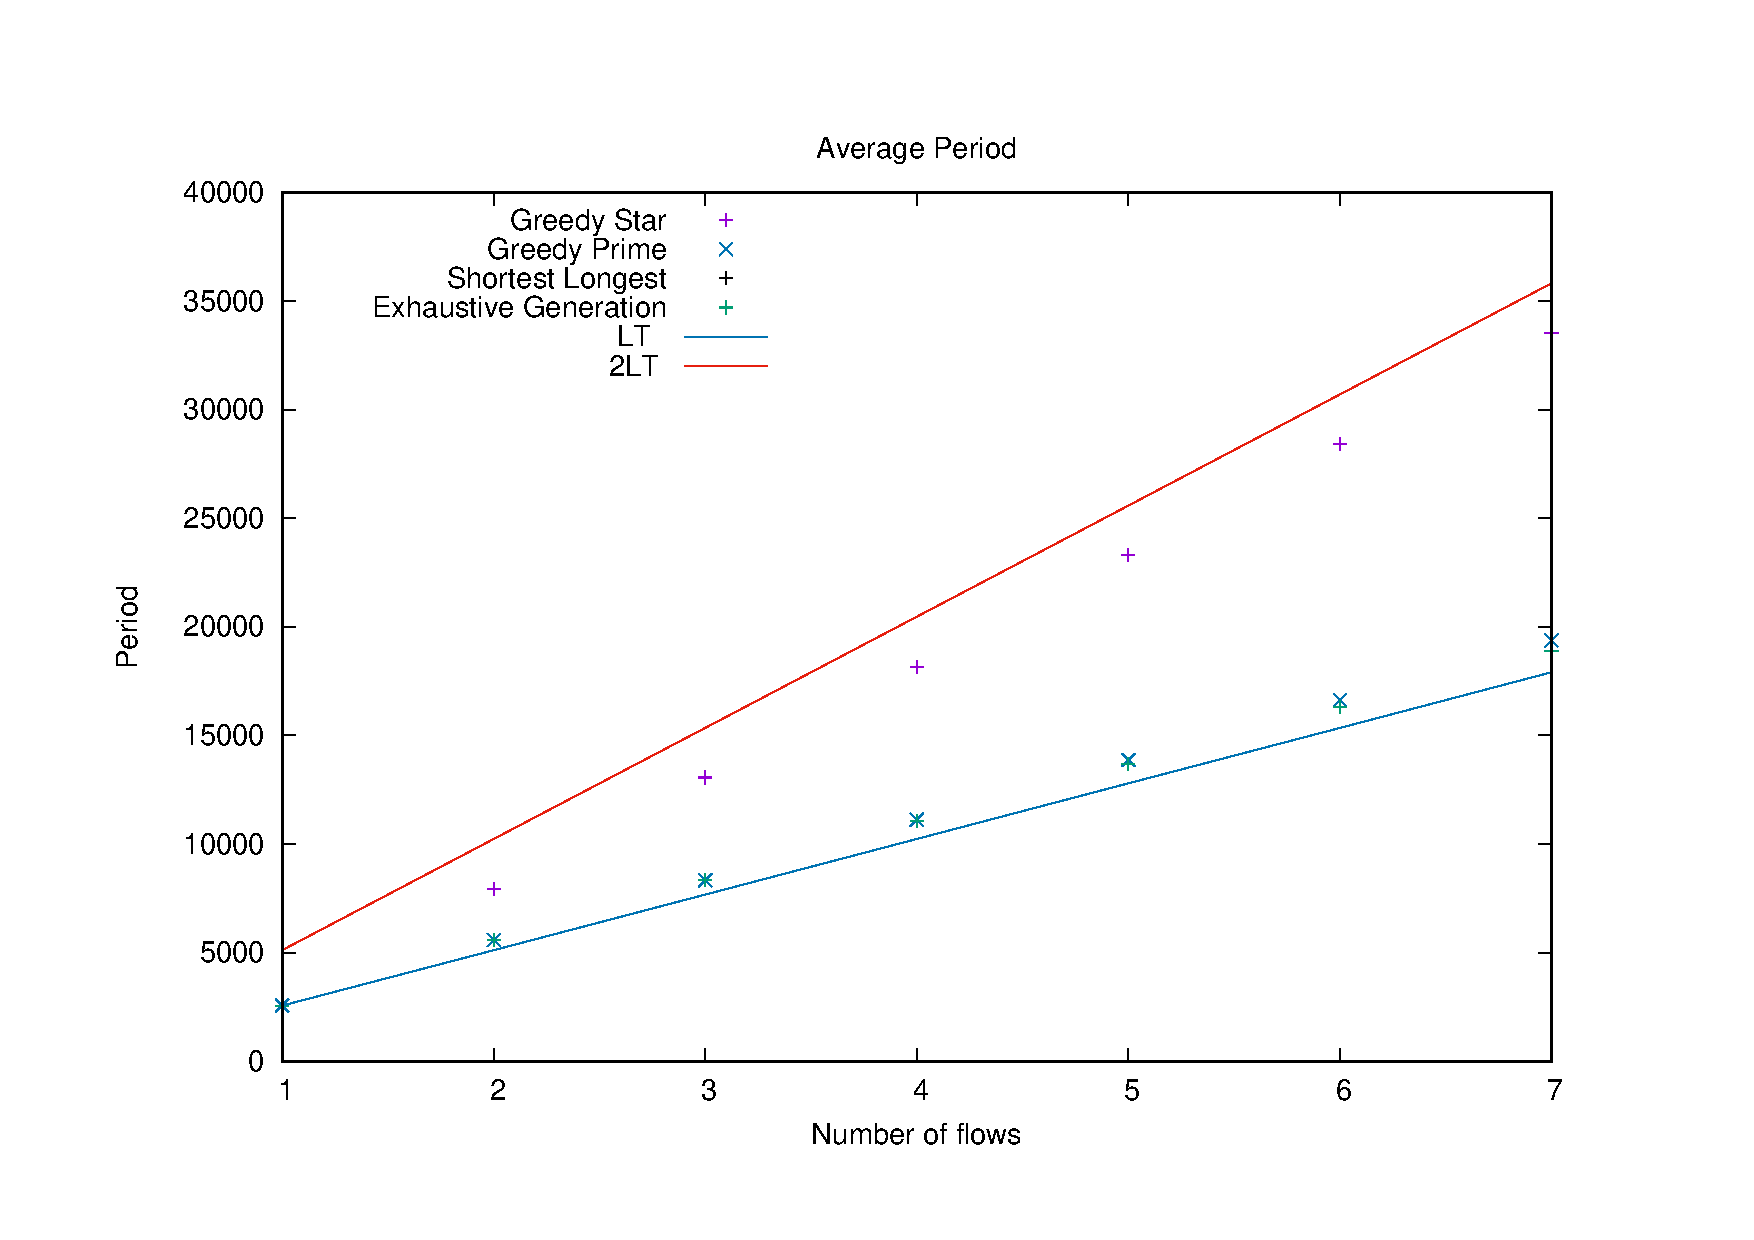
\includegraphics[scale=0.6]{window0.pdf}%scale=0.6
\caption{Average periods for algorithms without waiting times}
\end{figure}


Even if it has good theoretical insurances, the greedy star is not giving good solutions, as we can see, the average period for this algorithm is 
significantly high compared to the others.

The period given by the Shortest-longest is known and depends of the difference between the longest and the shortest route.
In this situation, this difference is never big enough to obtain bad periods. This algorithm is good in this situation but if we allow the 
route length to be greater, the period could significantly increase.

Greedy prime and bruteforce algorithms are finding solution in some very close average periods that are close to the lower bound.
That means those two algorithms are pretty good to find a solution without waiting time, but we will prefer the bruteforce,
because if a solution does not exists for a given graph and periods, using the bruteforce ensure us that the solution does really not exists.

The result is the same if we look at the worst period needed on the 10000 experiences to find a solution without waiting times (cf Appendix Fig 1).
\end{section}

\begin{section}{Limits of avoiding waiting times}
Too see in which circumstances finding a solution without waiting times is reasonable, we progressively increased the load of a network,
then we looked how many times the bruteforce algorithm is finding a solution for each flows.
We made this experience on a network composed of 16 flows max, on a period of 16 * 2500 slots.
The following figure is the result of a simulation made on 10000 experiences.

\begin{figure}[H]
\hspace*{-3cm}
\centering
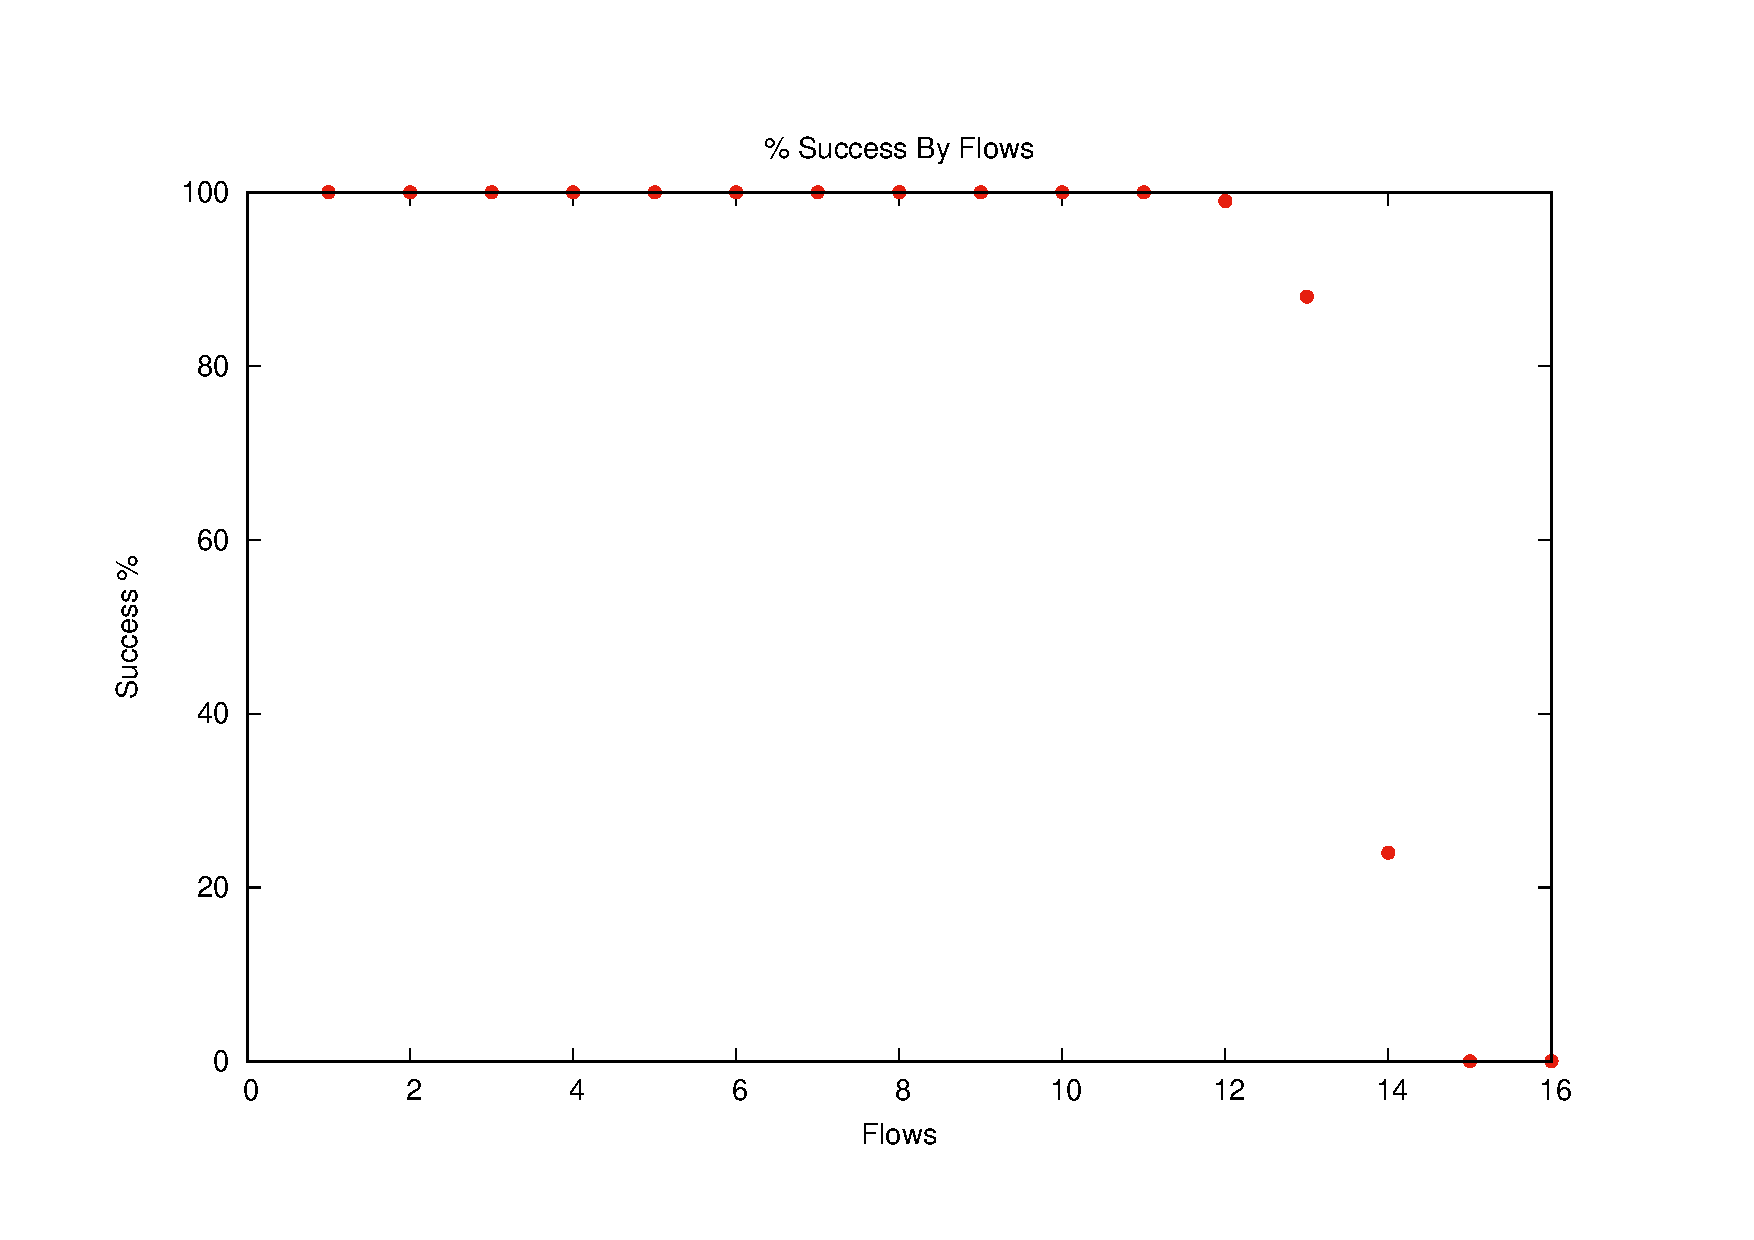
\includegraphics[scale=0.6]{expbruteforce.pdf}%scale=0.6
\caption{Success of Bruteforce by flows}
\end{figure}
As we can see, when the period is large enough according to the load, there is no problems. nevertheless, when we the load exceeds a certain limit 
($\simeq$85\%), the number of found solution decrease significantly.

In this situation, we have to find other options to find a solution : Allowing waiting times.

\end{section}

\begin{section}{Longest Shortest}

As we just noticed, it is not always possible to find a solution where the messages never wait anywhere in a given period.
The longest shortest allows us to find some solution in the smallest period (L*T), but does this algorithm ensure our maximum delay criteria ?
Does this algorithm change a lots on actual way to manage the messages through a network ?

\begin{subsection}{Simons and Longest-Shortest}
As we told it in the previous chapter, for our values, the simons and the longest-shortest algorithms are giving us the same results.

We made some simulation on 10000 graphs generated by the same way than in the previous section.
On those graphs, we applied the Longest shortest algorithm and the Simons algorithm, then we looked at the average and worst $T_{max}$.
As a reminder, $T_{max}$ is the longest time taken by a message to do the TwoWayTrip ( physical delay + waiting time).

As we can see in the Appendix Fig 2 and Fig 3, the results are strictly the same for the two algorithms. This is not surprising given the
theoretical explanations.

Therefore, in the following of the study, we'll just talk about the longest-shortest algorithm.
\end{subsection}


\begin{subsection}{Random sending}
Presently, the major part of the messages in a network are not really controlled; A message is sent and if they does not reach the destination,
they are re-sent until it is transmitted without loss. If many messages are crossing a same switch in the same times, some of them are buffered,
others are redirected or destroyed. This way to manage the message is maladjusted to our problem in which the latency constraints are strong.

Thus, we compared our results on the longest-shortest simulation with some random sending generated with the following laws : 
\begin{enumerate}
 \item The starting offsets are randomly generated, following a uniform law between 0 and P.
 \item If several messages are crossing a same switch in the same time, the first message pass and the others are buffered by arrival order.
\end{enumerate}

Then, we count the time for the messages to make the TwoWayTrip.
\end{subsection}

\begin{subsection}{Random against Longest-Shortest}
 
The following result shows us the difference of the average $T_{max}$ between the two algorithms.
The Orange points represent the random sending results, and the black points represent the longest-shortest results.
The blue circle are the average lower Bound i.e. the average size of twice the longest route in the generated graphs.
Indeed, if the $T_{max}$ of a solution is this size, that means the solution is optimal because this travel time is irreducible.

The red line is the Deadline. It represents the 0.4 ms maximum for a message to do the TwoWayTrip.

\begin{figure}[H]
\hspace*{-3cm}
\centering
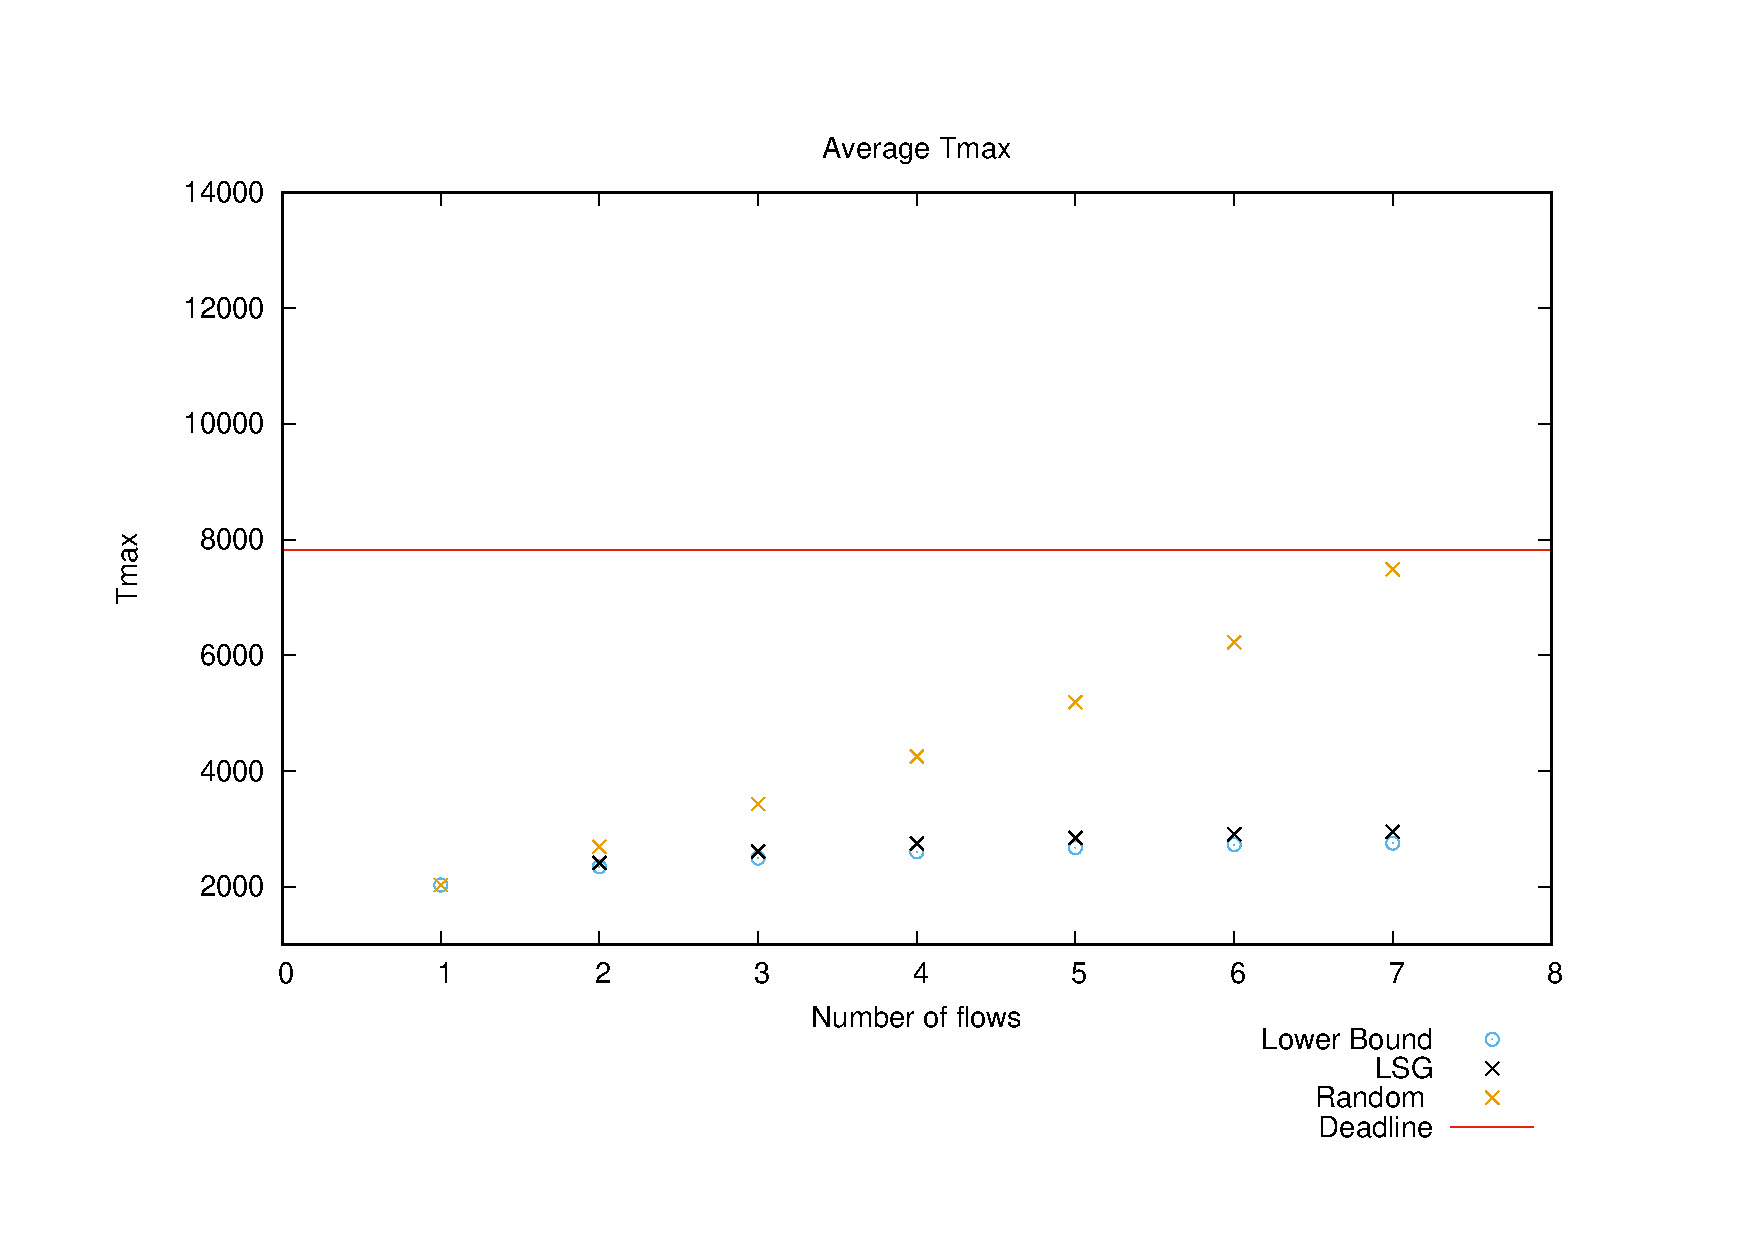
\includegraphics[scale=0.6]{tmax0.pdf}%scale=0.6
\caption{Average $T_{max}$ for the random sending and the longest-shortest deterministic sending.}
\end{figure}

The longest shortest gives us some good results, close from the lower bound expected. On the other hand, for the random sending, 
the greater the load of the network is, the greater the average $T_{max}$ are. When the network starts to be congested, the 
message managing politic generate a lot of latency by the buffering, so the $T_{max}$ significantly increase, until the deadline for 5 flows or more.


Also, the worst case shows us that with longest shortest, $T_{max}$ never exceed the deadline, while with the random sending, we obtain some
critical cases when the load is to 3 flows (Cf Appendix Fig 4).


The two following figures show us the distribution of the $T_{max}$ on 100 000 graphs using firstly the longest-shortest algorithm, then the
random sending.
Each curve represents the distribution of $T_{max}$ for a given number of flows.
\begin{figure}[H]
\hspace*{-4cm}
\centering
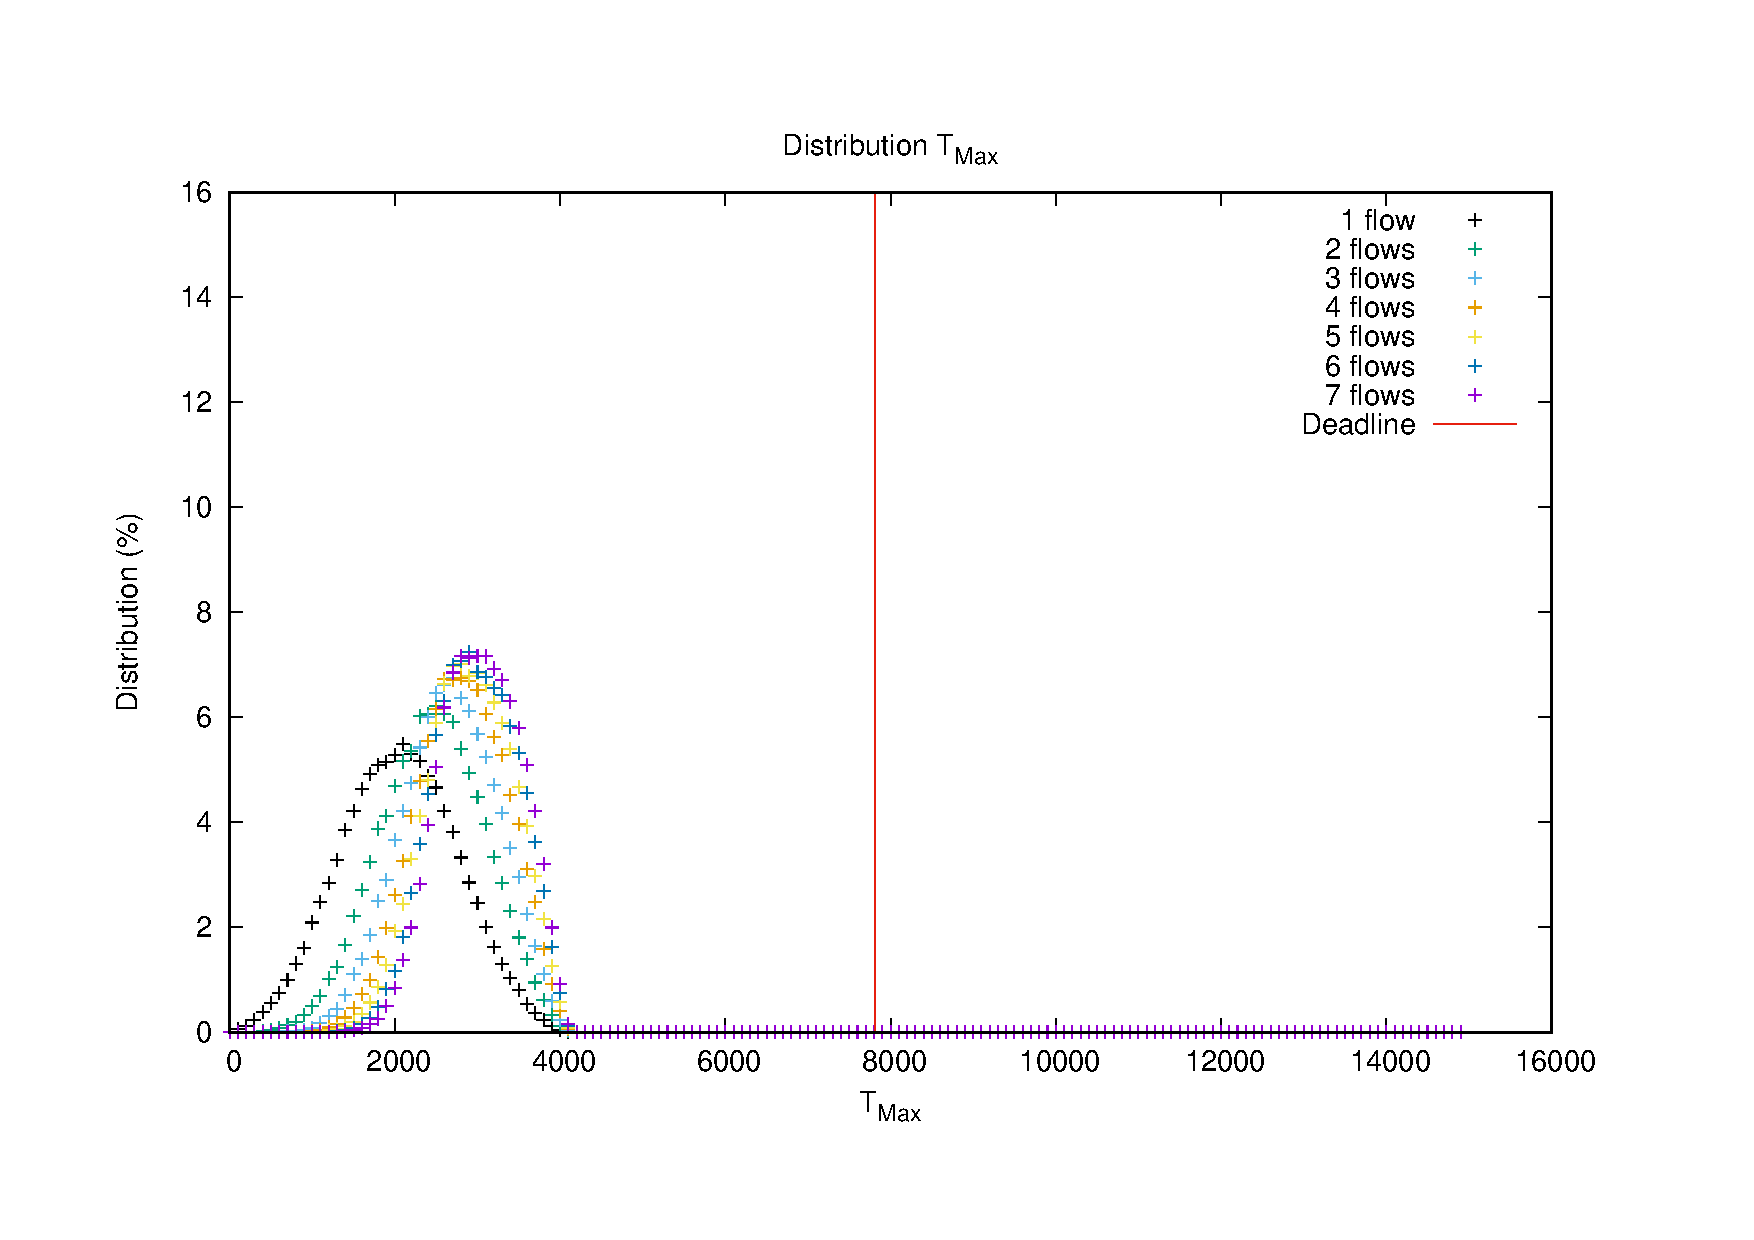
\includegraphics[scale=0.7]{distributions_longest.pdf}%scale=0.6
\caption{Distributions for longest-Shortest}
\end{figure}

\begin{figure}[H]
\hspace*{-3cm}
\centering
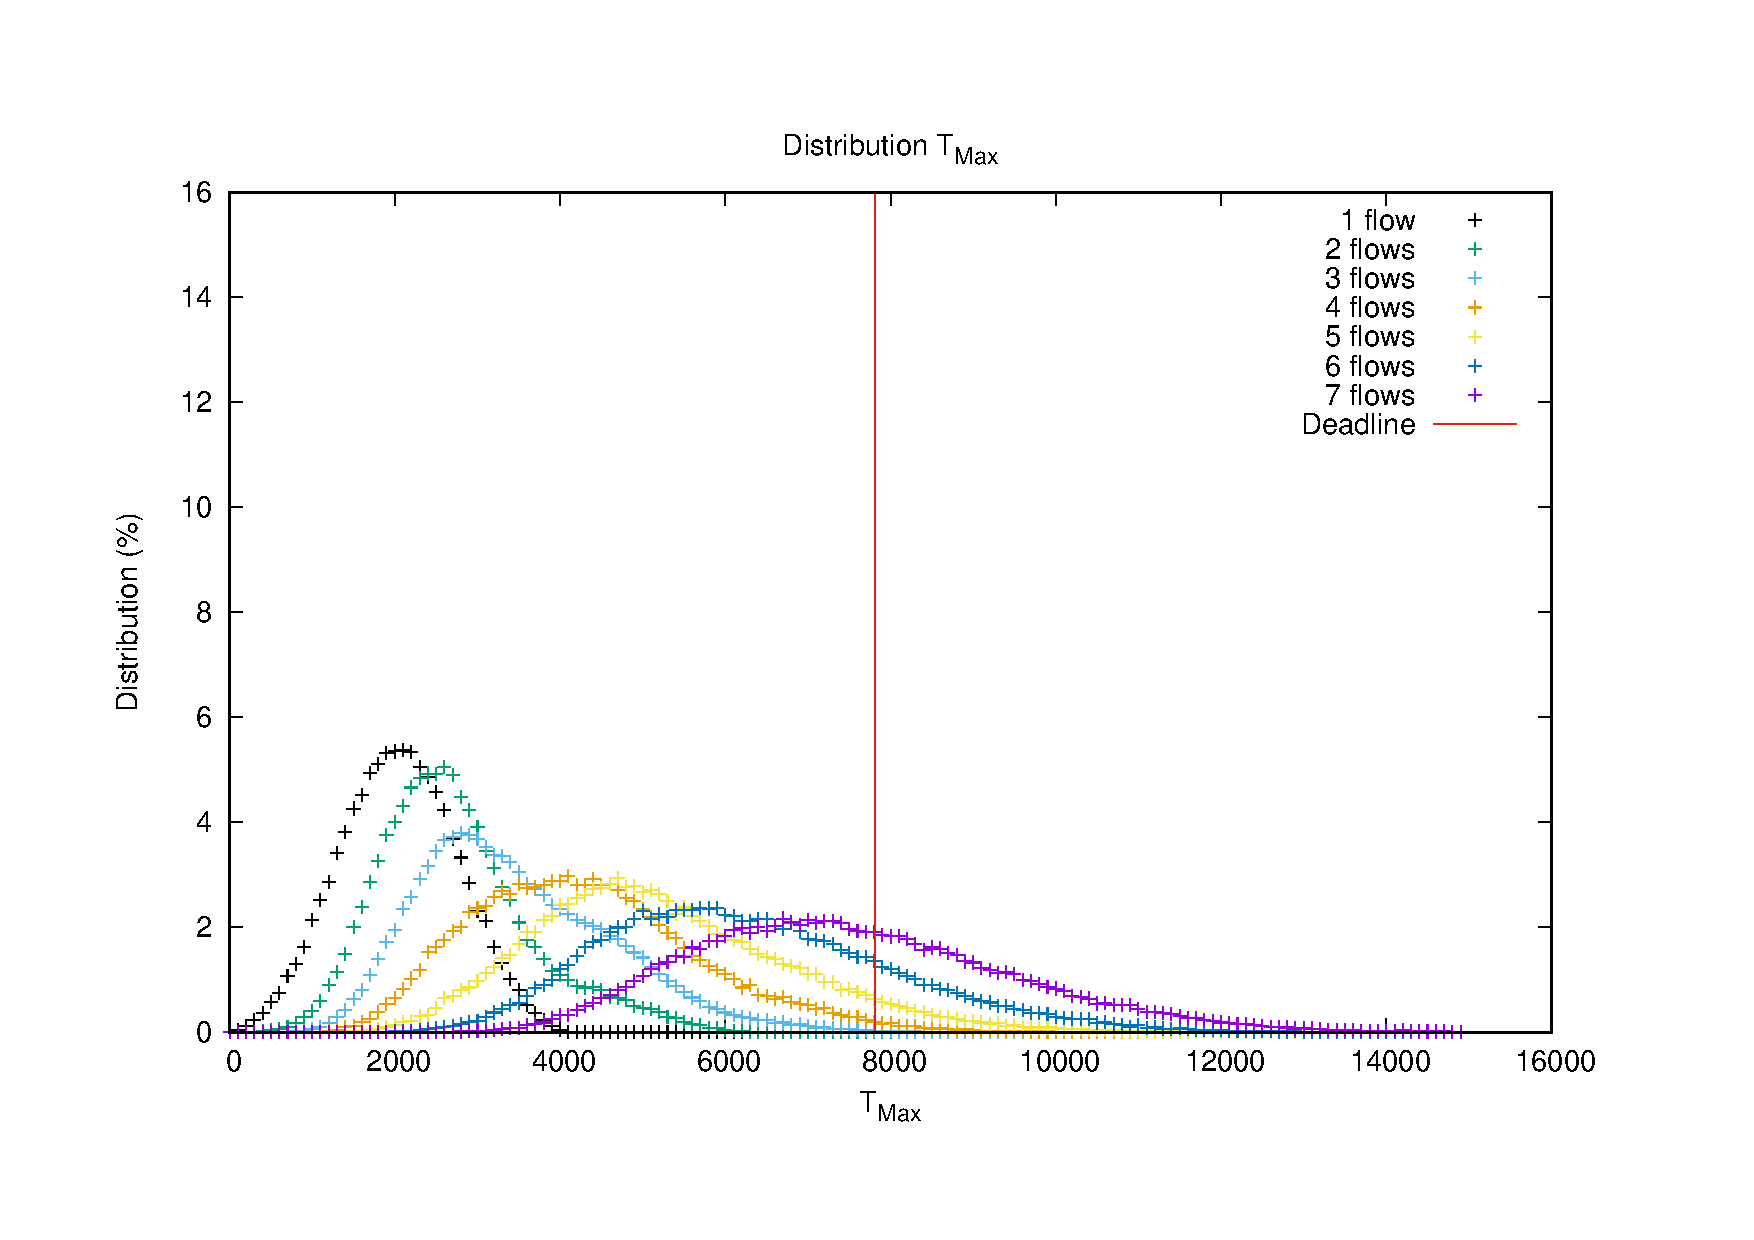
\includegraphics[scale=0.6]{distributions_random.pdf}%scale=0.6
\caption{Distributions For random}
\end{figure}

We recognise the previous results. For the longest shortest, the major part of the solutions are giving $T_{max} \simeq 2500-3000$, and there is no
solution with $T_{max}$ exceeding $\simeq 4000$ slots.
The random sending is giving more distributed results. A lot of cases gives us some $T_{max} >$ deadline for 3 flows or more.
The cumulative distribution (cf Appendix Fig 5 and 6) shows us that with 7 flows, we have $\simeq 60\%$ of the cases in which $T_{max} >$ deadline


\end{subsection}

\end{section}

\begin{section}{Synthesis}
Find a solution without waiting time would be the perfect option to solve our problem because it ensure us the minimal latency.

To find such a solution, we proposed four algorithms. The first one has theoretical certitudes but practical bad results (Greedy prime).
For the Shortest-Longest Algorithm we can calculate the period depending of the difference between the longest and the shortest route.
In our situation, this algorithm gives us good results because that difference is not that great.
Then, the greedy prime algorithm and the bruteforce find some good solutions close to the lower bound in the same average period.
However, the bruteforce ensure us to find a solution if it exists, while the greedy prime can fails.

Furthermore deleting all the buffers involve to get a large enough window. Considering our problem, we noticed that when the 
load increase, there is a lot of cases in which a solution without waiting time does not exists.

Thus, by allowing the messages to be buffered in source nodes with the longest-shortest algorithm, we find good solutions responding to our latency 
criteria in the given period. To prove that this algorithm is useful, we compared the results of the longest shortest with the results of some
random messages sending managed with some buffers in switches. The results have proven that the longest shortest is firmly useful, if we want
to satisfy the latency constraint.

\end{section}

\end{chapter}



\begin{chapter}{Conclusion}

This study took place in a collaboration between Nokia Bell Labs France and DAVID laboratory.
A previous work about the study of the complexity of the general case (topology 3) was made before my work.
In the first month, the principal objective was to define the problem with the specifications corresponding to the reality.
In parallel, we started to study some related works and to try finding some roots. That is the reason why some articles are not related
with the first topology on which we worked in that study, but on the current case.

The precise definition of this problem opened a lot of questions on the first topology, that is why we only studied it.

Then we proposed a first approach to solve this scheduling problem, without considering waiting times. We saw with the simulations 
that this approach gives us satisfying results until the load of the network is not too raised.
The second approach, which is to allow waiting time and to find a good heuristic to schedule the messages respecting the latency constraints,
gave us good solution, compared to experimental traditional sending, that correspond to nowadays way to manage the network.

\todo{regarder un peu l'anneau de voir si on ne peut pas réutiliser certaines propriétées}


\end{chapter}
\appendix

\chapter*{Appendix}
\addcontentsline{toc}{chapter}{Appendix}

 
\begin{figure}[H]
\hspace*{-3cm}
\centering
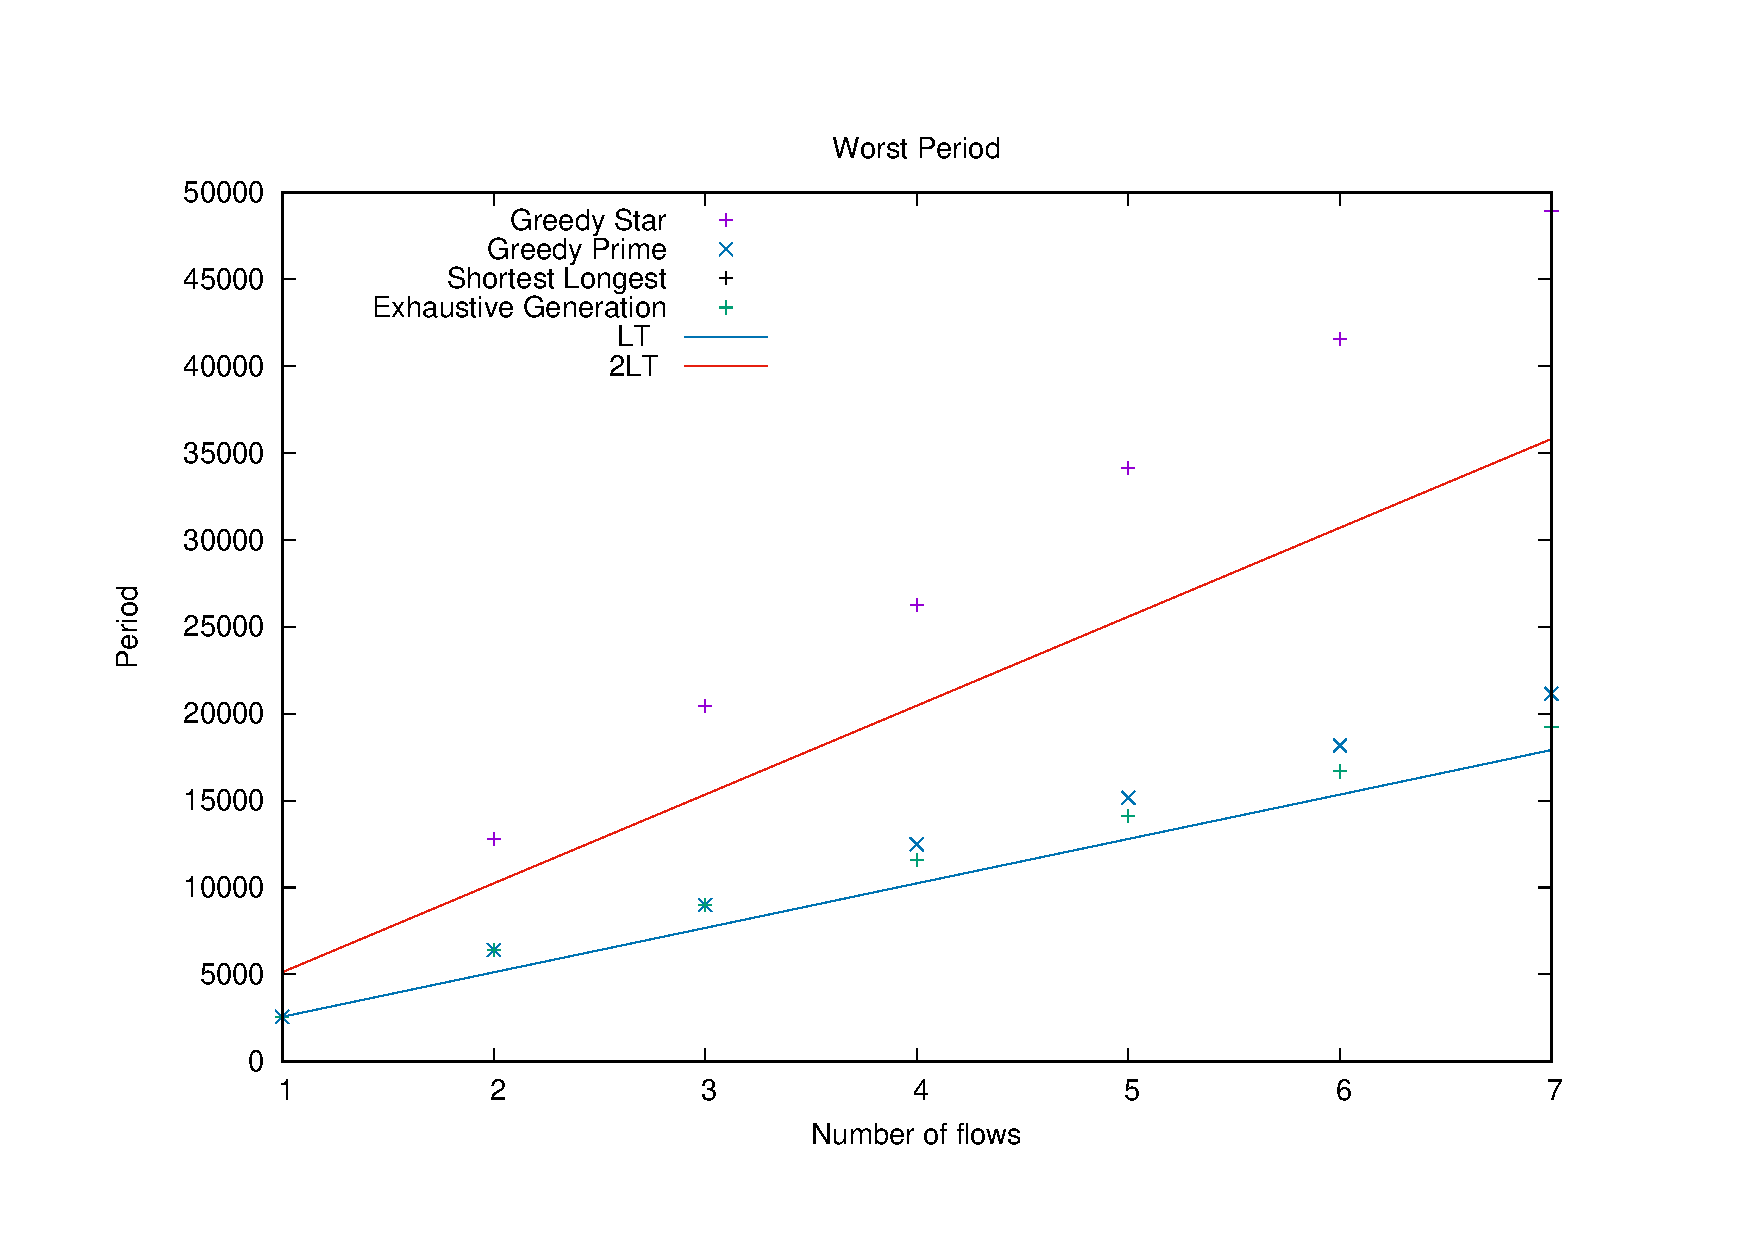
\includegraphics[scale=0.6]{windowworst.pdf}%scale=0.6
\caption{Worst periods for algorithms without waiting times}
\end{figure}

\begin{figure}[H]
\hspace*{-3cm}
\centering
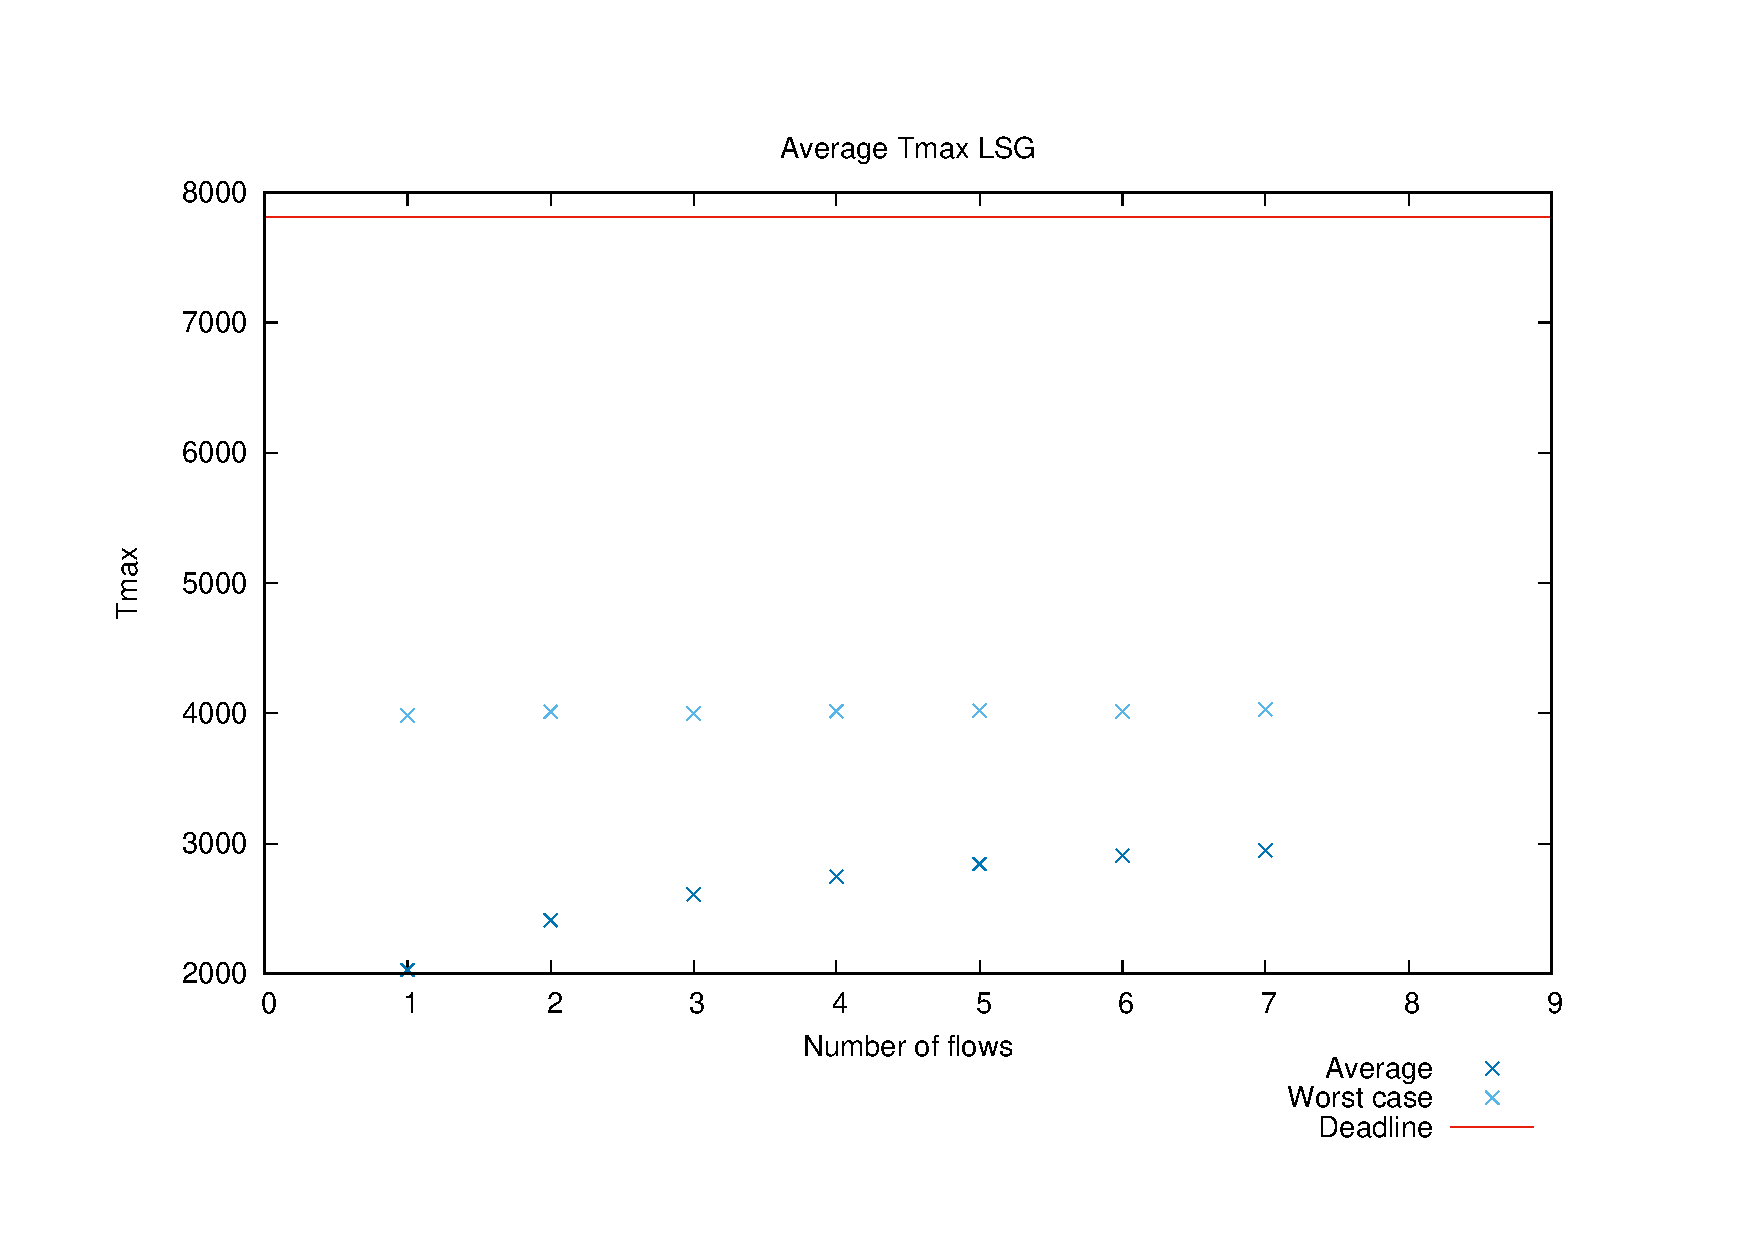
\includegraphics[scale=0.6]{tmaxlongest.pdf}%scale=0.6
\caption{$T_{max}$ with Longest shortest}
\end{figure}

\begin{figure}[H]
\hspace*{-3cm}
\centering
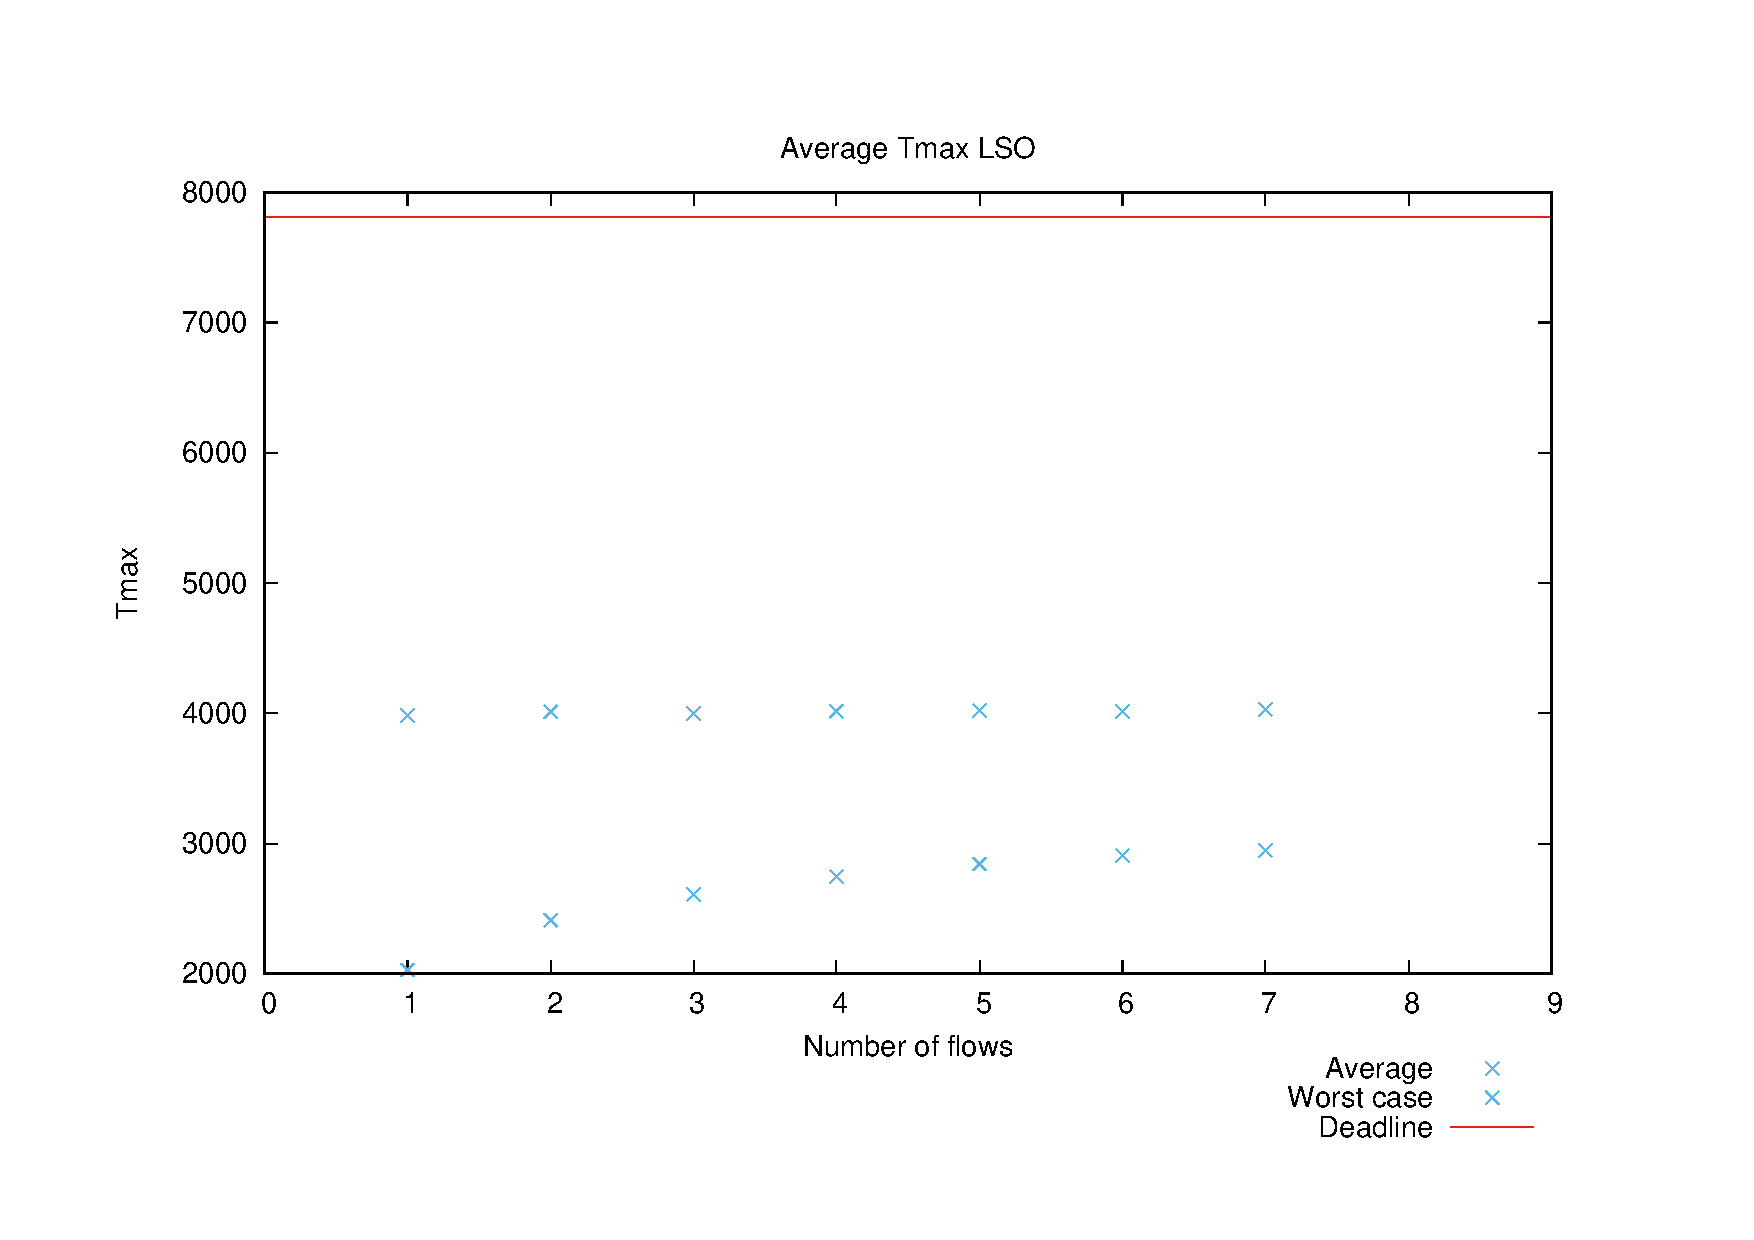
\includegraphics[scale=0.6]{tmaxsimons.pdf}%scale=0.6
\caption{$T_{max}$ with Simons}
\end{figure}


\begin{figure}[H]
\hspace*{-3cm}
\centering
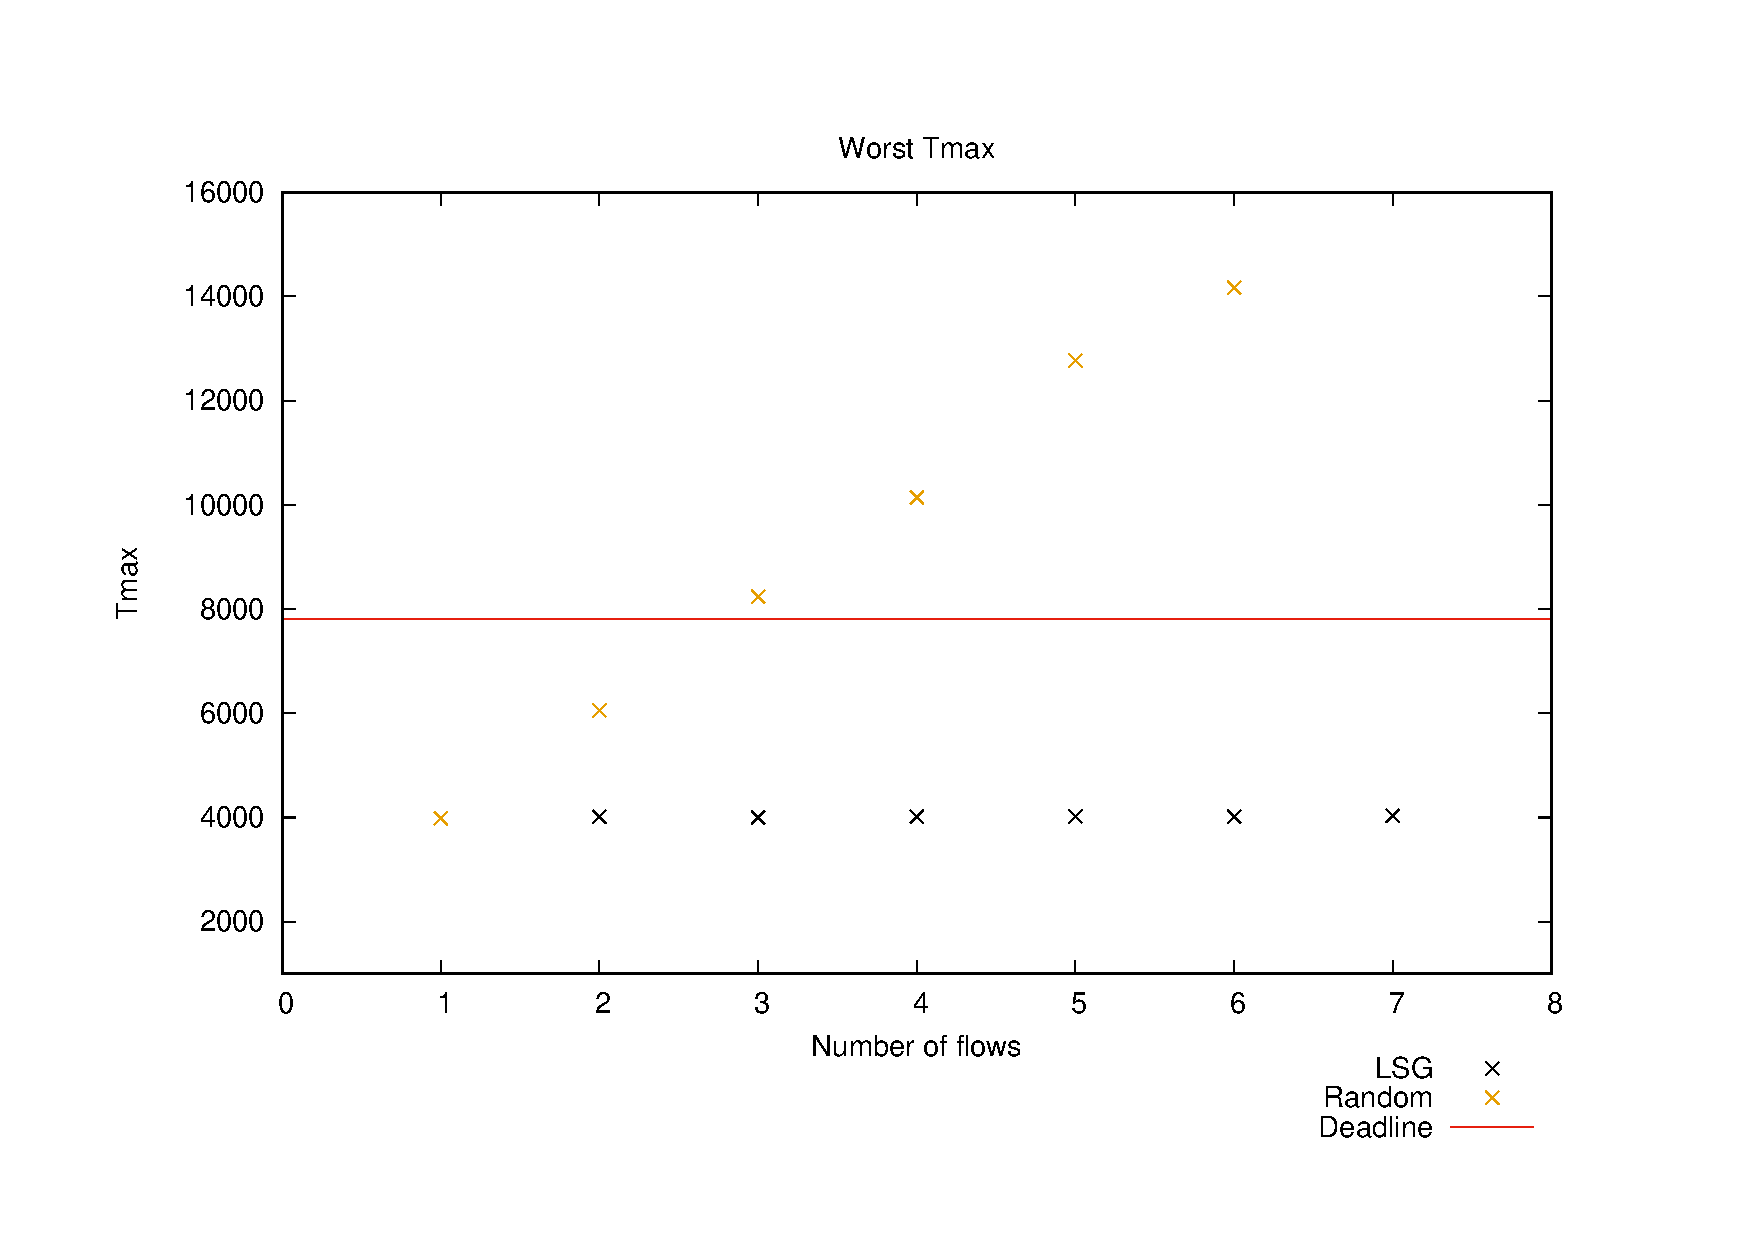
\includegraphics[scale=0.6]{tmax0worst.pdf}%scale=0.6
\caption{Worst $T_{max}$ with Random and Longest Shortest}
\end{figure}


\begin{figure}[H]
\hspace*{-3cm}
\centering
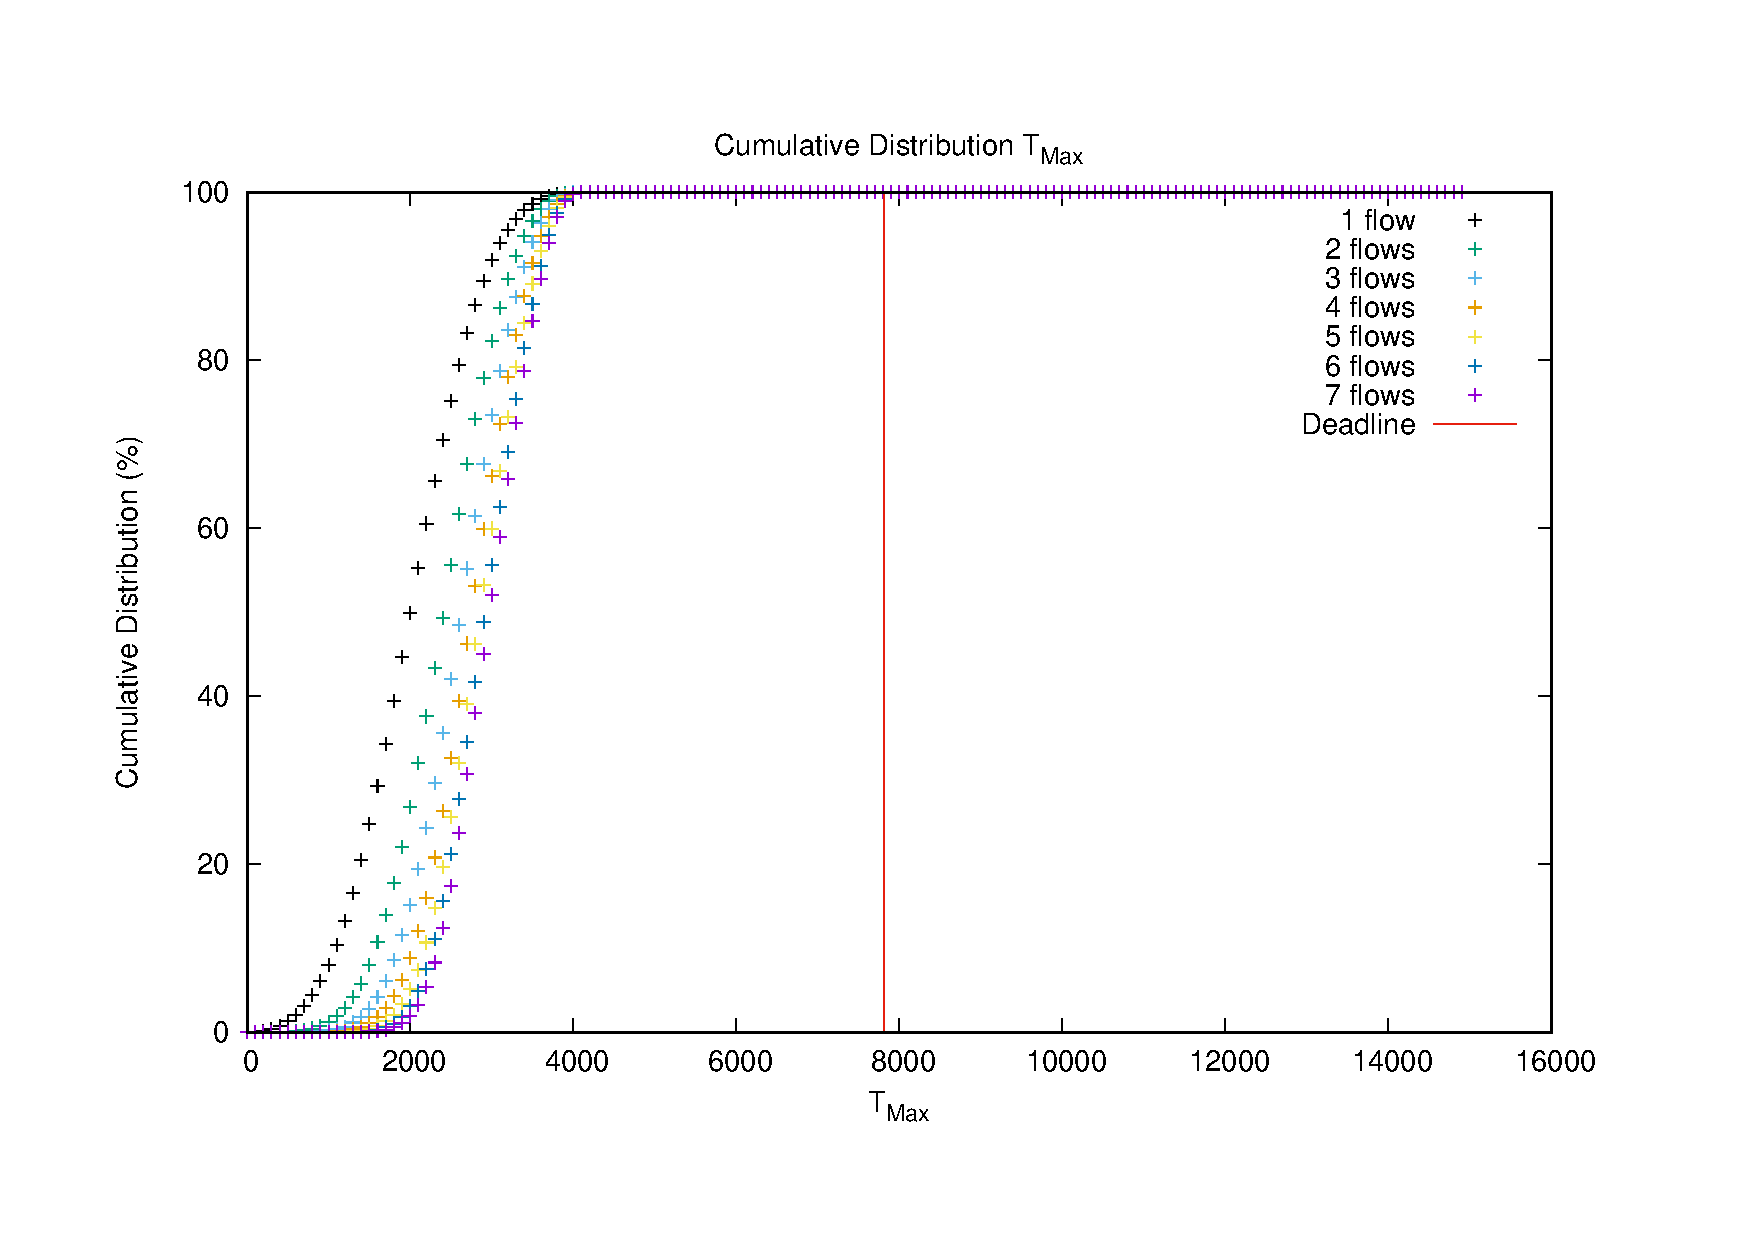
\includegraphics[scale=0.6]{distriscumul_longest.pdf}%scale=0.6
\caption{Cumulative distributions For Longest-Shortest}
\end{figure}

\begin{figure}[H]
\hspace*{-3cm}
\centering
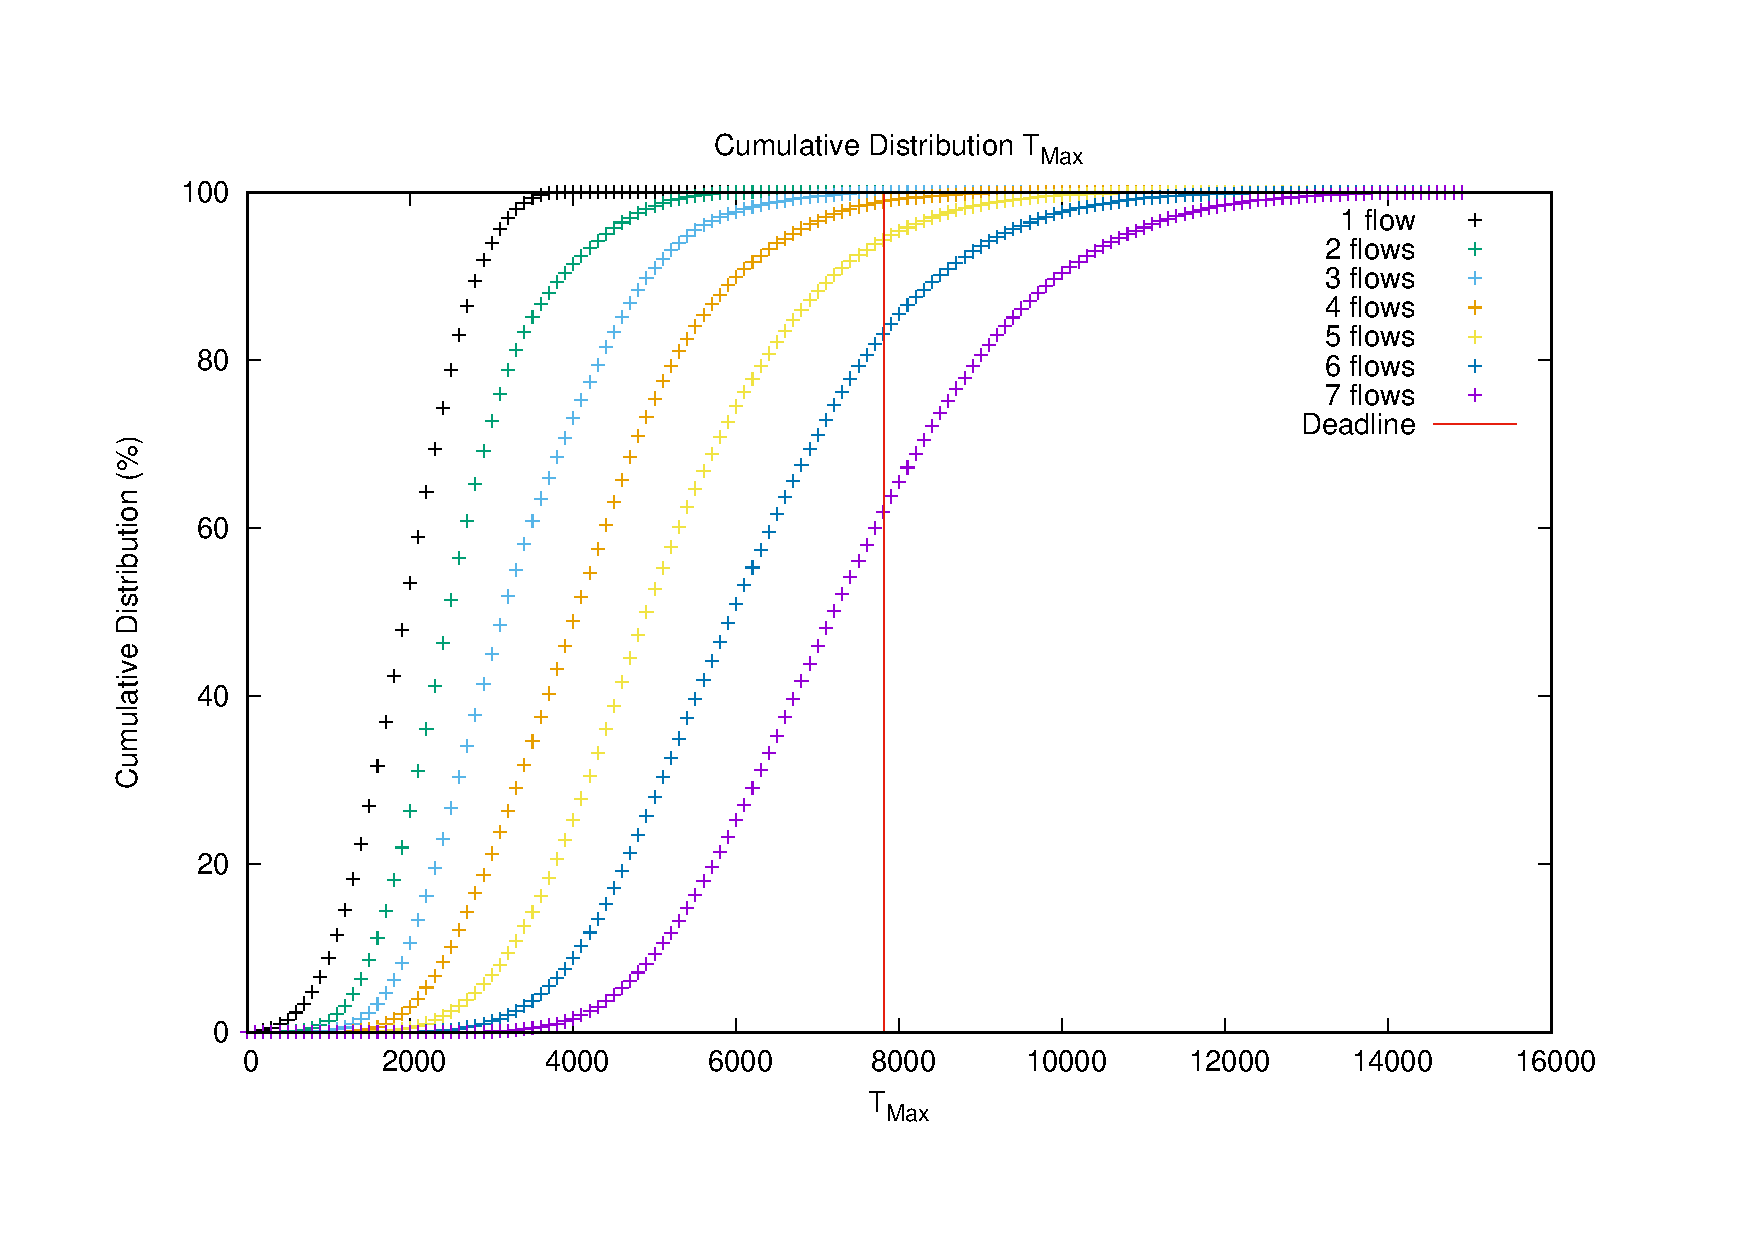
\includegraphics[scale=0.6]{distriscumul_random.pdf}%scale=0.6
\caption{Cumulative distributions For Random}
\end{figure}


\bibliographystyle{plain}
\bibliography{Sources}
\addcontentsline{toc}{chapter}{Bibliography}
\end{document}
